\chapter{Combination inference}
\label{sec:comb:combination}
\setstretch{\lspac}

% IUT
% Conjunction/disjunction
% partial, marginal
% F-tests, rejection regions
% FWER 
% Meta-analysis
% Diagram, comparison
% Relationship with cognition, biological interpretation

% Implementation aspects: avoid being close to 1, etc
% Common framework for different tests

% Uses of NPC
% - Different modalities
% - Same modality, different aspects -- ICs, DTI scalars, thick/area
% - Repeated measurements
% - Non-orthogonal studies

% Philosophical questions: should we combine or dissect?

\section{Introduction}
\label{sec:comb:intro}

In this paper we show that permutation tests can provide a common solution to seemingly disparate problems that arise when dealing with multiple imaging measurements. These problems refer to the multiplicity of tests, and to the combination of information across multiple modalities for joint inference. We begin by describing each of these problems separately, then show how they are related, and offer a complete and generic solution that can accommodate a myriad of designs that can mix imaging and non-imaging data. We also present an algorithm that has with amenable computational demands for treating these problems.

\subsection{Multiple tests --- but not the usual multiplicity}

Because in neuroimaging one statistical test is typically performed at each of many thousands of imaging units (e.g., voxels or vertices), the problems related to such multiplicity of tests were recognised almost as early as these techniques were developed \citep[for pioneering examples, see][]{Fox1988, Friston1991}. There is now a comprehensive body of literature on multiple testing correction methods that include those based on the random field theory, on permutation tests, as well as on other strategies that control the familywise error rate (\textsc{fwer}) or the false discovery rate (\textsc{fdr}) \citep[for reviews, see][]{Nichols2003, Nichols2012}. However, the multiplicity of tests in neuroimaging can appear in other ways that are less explicit, and most importantly, that have not been fully appreciated or made available in software packages. In the context of the general linear model \citep[\textsc{glm},][]{Scheffe1959}, these \emph{other} multiple tests include:

\renewcommand{\theenumi}{\textsc{\alph{enumi}.}}
\begin{enumerate}[leftmargin=*]
\item \emph{Multiple hypotheses in the same model:} Testing more than one hypothesis regarding a set of explanatory variables. An example is testing the effects of multiple variables, such as presence of a disease along with its duration, some clinical score, age and/or sex of the subjects, on a given imaging measurement, such as maps from functional magnetic resonance imaging (\textsc{fmri}) experiments.
\item \emph{Multiple pairwise group comparisons:} Often an initial global (omnibus) test is performed, such as an $F$-test in the context of analysis of variance (\textsc{anova}), and if this test is significant, subsequent (post hoc) tests are performed to verify which pairwise difference(s) drove the global result, thus introducing a multiple comparisons problem.
\item \emph{Multiple models:} Testing more than one set of explanatory variables on one given dataset, that is, assembling and testing more than one design matrix, each with its own set of regressors, which may differ across designs, and each with its own set of contrasts. An example is interrogating the effect of distinct seeds, one at a time, in a resting-state \textsc{fmri} experiment; another is in an imaging genetics experiment, testing multiple candidate polymorphisms.
\item \emph{Multiple modalities:} Testing separately, in the same study, more than one imaging modality as the response variable, such as \textsc{fmri} and positron-emission tomography (\textsc{pet}), or different metrics from the same modality, such as various measurements from diffusion tensor imaging (\textsc{dti}), as fractional anisotropy (\textsc{fa}), mean diffusivity (\textsc{md}), or radial diffusivity (\textsc{rd}), or the effect of various networks identified using independent component analysis (\textsc{ica}).
\item \emph{Imaging and non-imaging:} Testing separately, in the same study, imaging and non-imaging measurements as response variables. An example is studying group effects on \textsc{fmri} and on behavioural or cognitive scores, such as \textsc{iq}, or disease severity scores, among countless other non-imaging measurements.
\item \emph{Multiple processing pipelines:} Testing the same imaging modality multiple times, each time after a different processing pipeline, such as using filters with different widths for smoothing, or using different strategies for registration to a common space.
\item \emph{Multiple multivariate analyses:} Testing more than one multivariate hypothesis with the \textsc{glm} in repeated measurements designs, such as in profile analyses, in which the same data allows various different hypotheses about the relationships between explanatory and response variables.
\end{enumerate}
\renewcommand{\theenumi}{\arabic{enumi}.}

In all these cases, the multiple tests cannot be assumed to be independent, so that the simple \textsc{fwer} correction using the conventional Bonferroni method risks a considerable loss in power. Modelling the degree of dependence between these tests can be a daunting task, and be suboptimal by invariably requiring the introduction of assumptions about the data, which, if at all valid, may not be sufficient. By contrast, robust, generic, multi-step procedures, which do not depend as much on assumptions, or on independence among tests, such as the Benjamini--Hochberg procedure that controls the false discovery rate (\textsc{fdr}) \citep{Benjamini1995, Genovese2002}, do not guarantee that the spatial relationship between voxels or vertices within test is preserved when applied across \emph{these} multiple tests, therefore being not as useful as in other settings. More specifically, the difficulty relates to correcting across various distinct imaging tests, while maintaining control across space within any given test, as opposed to controlling just within a single imaging test as commonly done. For the same reason, various multiple testing approaches that are applicable to many particular cases, can hardly be used for the problems we discuss here; extensive details on these tests can be found in \citet{Hochberg1987} and in \citet{Hsu1996}.

We call the multiple tests that arise in situations as those listed above ``multiple testing problem \textsc{ii}'' (\textsc{mtp-ii}), to allow a distinction from the usual multiple testing problem due to the many voxels/vertices/faces that constitute an image, which we denote ``multiple testing problem \textsc{i}'' (\textsc{mtp-i}). Methods that can be used in neuroimaging for the \textsc{mtp-i} not always can be considered for the \textsc{mtp-ii}, a problem that has remained largely without treatment; for two rare counter examples in which the \textsc{mtp-ii} \emph{was} considered, we point to the studies by \citet{Licata2013} and \citet{AbouElseoud2014}.

\subsection{Combination of imaging modalities}
\label{sec:comb:fusion}

Acquisition of multiple imaging modalities on the same subjects can allow the examination of more complex hypotheses about physiological processes, and has potential to increase power to detect group differences. Such combination of modalities can refer strictly to data acquired from different instruments (e.g., \textsc{mri}, \textsc{pet}, \textsc{eeg}), or more broadly, to data acquired from the same instrument using different acquisition parameters (e.g., different \textsc{mri} sequences, different \textsc{pet} ligands); for an overview, see \citet{Uludag2014,Zhu2014}, and for example applications, see \citet{Hayasaka2006, Thomas2015}. Irrespective of which the modalities are, the options in the context of the \textsc{glm} rest in testing for a single multivariate hypothesis, or in testing for a combination of multiple univariate hypotheses. Single multivariate tests encompass various classical tests, known in particular cases as multivariate analysis of variance (\textsc{manova}), multivariate analysis of covariance (\textsc{mancova}), or canonical correlation/variates analysis (\textsc{cca}/\textsc{cva}); these tests will be referred here as \emph{classical multivariate tests}, or \textsc{cmv}.

The combination of multiple univariate hypotheses requires that each is analysed separately, and that these results are grouped together to test, at each voxel (or vertex, or face) a \emph{joint null hypothesis} (\textsc{jnh}); in this context, the separate tests are termed \emph{partial tests}. Different criteria to decide upon rejection of the \textsc{jnh} give rise to three broad categories of combined tests: (\textsc{i}) reject if \emph{any} partial test is significant; (\textsc{ii}) reject if \emph{all} partial tests are significant; and (\textsc{iii}) reject if some \emph{aggregate measure} from the partial tests is significant. The first of these can be traced back to \citet{Tippett1931}, and in current terminology, could be defined as rejecting the joint null hypothesis if any partial test is rejected at the \textsc{fwer} level using the \v{S}id\'{a}k correction \citep{Sidak1967}; it also corresponds to a \emph{union--intersection test} \citep[\textsc{uit},][]{Roy1953}. The second is the \emph{intersection--union test} \citep[\textsc{iut},][]{Berger1982}, that in neuroimaging came to be known as \emph{conjunction test} \citep{Nichols2005}. The third offers a trade-off between the two other approaches, and gives rise to a large number of possible tests, each with a different rejection region, and therefore with different sensitivity and specificity profiles; some of these tests are popular in meta-analyses, with the method of Fisher \citep{Fisher1932} being one of the most popular, and new approaches are continually being developed. A summary is shown in Table~\ref{tab:comparison}, and a brief overview of these and yet other tests, along with bibliographic information, is in \ref{sec:comb:review}.

\begin{table}[!b]
\caption{\emph{(page \pageref{tab:comparison_noref})} Various functions are available for joint inference on multiple tests. For each method, both its statistic ($T$) and associated p-value, $P$ are shown. These p-values are only valid if, for each method, certain assumptions are met, particularly with respect to the independence between tests, but sometimes also with respect to underlying distributions. Under exchangeability, the p-values can be computed using permutation tests, and the formul\ae{} in the last column are no longer necessary. The tests are shown in chronological order; see \ref{sec:comb:review} for details and bibliographic information. In the table, 
$T$ is the statistic for each method and $P$ its asymptotic p-value. All methods are shown as function of the p-values for the partial tests. For certain methods, however, the test statistic for the partial tests, if available, can be used directly.
$K$ is the number of tests being combined,
$p_{k}$, $k=\left\{1,2,\ldots,K\right\}$ are the partial p-values,
$w_{k}$ are positive weights assigned to the respective $p_{k}$,
$p_{(r)}$ are the $p_{k}$ with rank $r$ in ascending order (most significant first),
$\alpha$ is the significance level for the partial tests,
%$v$ is the minimum number of tests where the null should be rejected for a partial conjunction null test,
$I(\cdot)$ is an indicator function that evaluates as 1 if the condition is satisfied, 0 otherwise,
$\lfloor \cdot \rfloor$ represents the floor function,
$\chi^{2}_{\nu}$ is the cumulative distribution function (cdf) for a $\chi^{2}$ distribution, with the $\nu$ degrees of freedom,
$t_{\text{cdf}}$ is the cdf of the Student's $t$ distribution with degrees of freedom $\nu$, and $t_{\text{cdf}}^{-1}$ its inverse,
$\Phi$ is the cdf of the normal distribution with mean $\mu$ and variance $\sigma^{2}$, and $\Phi^{-1}$ its inverse, and
$F$ and $G$ are the cdf of arbitrary, yet well chosen distributions.
For the two Dudbridge--Koeleman methods, $A\left(T,a,b\right)=I\left(T>a^{b}\right) a^{b} +I\left(T \leqslant a^{b}\right) T \sum_{j=0}^{b-1}{\left(b\ln a - \ln T\right)^{j}}/{j!}$.}
\label{tab:comparison}
\end{table}
\addtolength{\belowcaptionskip}{-0pt}
\begin{sidewaystable}
\begin{center}
{\footnotesize
\begin{tabular}{@{}m{4.3cm}@{}m{5.7cm}<{\raggedright}@{}m{12.2cm}<{\raggedright}@{}}
\toprule
\textbf{Method} & \textbf{Test statistic ($T$)} & \textbf{p-value ($P$)}\\
\midrule
Tippett &
$\min \left(p_{k}\right)$ &
$1-\left(1-T\right)^{K}$ \\
\midrule[0pt]
Fisher &
$-2 \sum_{k=1}^{K} \ln\left(p_{k}\right)$ &
$1-\chi^{2}\left(T;\;\nu=2K\right)$\\
\midrule[0pt]
Stouffer &
$\frac{1}{\sqrt{K}} \sum_{k=1}^{K} \Phi^{-1}\left(1-p_{k}\right)$ &
$1-\Phi\left(T;\;\mu=0,\;\sigma^2=1\right)$\\
\midrule[0pt]
Wilkinson &
$\sum_{k=1}^{K} I\left(p_{k}\leqslant\alpha\right)$ &
$\sum_{k=T}^{K}\binom{K}{k}\alpha^{k}(1-\alpha)^{K-k}$ \\
\midrule[0pt]
Good &
$\prod_{k=1}^{K} p_{k}^{w_{k}}$ &
$\sum_{k=1}^{K}w_{k}^{K-1}T^{1/w_{k}}\left(\prod_{i=1}^{k-1}\left(w_{k}-w_{i}\right)^{-1}\right) \left(\prod_{i=k+1}^{K}\left(w_{k}-w_{i}\right)^{-1}\right)$\\
\midrule[0pt]
Lancaster &
$\sum_{k=1}^{K} w_{k}F_{k}^{-1}\left(1-p_{k}\right)$ &
$1-G\left(T\right)$\\
\midrule[0pt]
Winer &
$\sum_{k=1}^{K}t_{\text{cdf}}^{-1}\left(1-p_{k};\;\nu_{k}\right)\left/\sqrt{\sum_{k=1}^{K}\frac{\nu_{k}}{\nu_{k}-2}}\right.$ &
$1-\Phi\left(T;\;\mu=0,\;\sigma^2=1\right)$\\
\midrule[0pt]
Edgington &
$\sum_{k=1}^{K} p_{k}$& 
$\sum_{j=0}^{\lfloor T \rfloor}(-1)^j \binom{K}{j}\frac{\left(T-j\right)^K}{K!}$ \\
\midrule[0pt]
Mudholkar--George &
$\frac{1}{\pi}\sqrt{\frac{3(5K+4)}{K(5K+2)}}\sum_{k=1}^{K} \ln\left(\frac{1-p_{k}}{p_{k}}\right)$ &
$1-t_{\text{cdf}}(T;\;\nu=5K+4)$\\
\midrule[0pt]
%Friston &
%$\max \left(p_{k}\right)$ &
%$T^{K}$ (global null) or $T^{K-v+1}$ (partial conjunction null)\\
%\midrule[0pt]
Darlington--Hayes &
$\frac{1}{r} \sum_{k=1}^{r} \Phi^{-1}\left(1-p_{(k)}\right)$ &
Computed through Monte Carlo methods. Tables are available.\\
\midrule[0pt]
Zaykin et al.\ (\textsc{tpm}) &
$\prod_{k=1}^{K} p_{k}^{I\left(p_{k} \leqslant \alpha\right)}$ &
$\sum_{k=1}^{K}\binom{K}{k}\left(1-\alpha\right)^{K-k}\left(I\left(T> \alpha^{k}\right) \alpha^{k}  + I\left(T\leqslant \alpha^{k}\right)T\sum_{j=0}^{k-1}\frac{\left(k\ln \alpha - \ln T\right)^{j}}{j!}\right)$\\
\midrule[0pt]
Dudbridge--Koeleman (\textsc{rtp}) &
$\prod_{k=1}^{r} p_{(k)}$ &
$\binom{K}{r+1}\left(r+1\right) \int_0^1\left(1-t\right)^{K-r-1}A\left(T,t,K\right)\mathrm{d}t$ \\
\midrule[0pt]
Dudbridge--Koeleman (\textsc{dtp}) &
$\max\left(\prod_{k=1}^{r} p_{(k)},\prod_{k=1}^{K} p_{k}^{I\left(p_{k} \leqslant \alpha\right)}\right)$ &
$\sum_{k=1}^{r}\binom{K}{k}\left(1-\alpha\right)^{K-k}A\left(T,\alpha,k\right) + I\left(r \! < \! K\right)\binom{K}{r+1}\left(r+1\right) \int_{0}^{\alpha}\left(1-t\right)^{K-r-1}A\left(T,t,K\right)\mathrm{d}t$ \\
\midrule[0pt]
Taylor--Tibshirani (\textsc{ts}) &
$\frac{1}{K} \sum_{k=1}^{K} \left(1-p_{(k)}\frac{K+1}{k}\right)$ &
$1-\Phi\left(T;\;\mu=0,\;\sigma^2 \approx \frac{1}{K}\right)$ \\
\midrule[0pt]
Jiang et al.\ (\textsc{tts}) &
$\frac{1}{K} \sum_{k=1}^{K} I\left(p_{(k)}\leqslant \alpha \right)\left(1-p_{(k)}\frac{K+1}{k}\right)$ &
Computed through Monte Carlo methods.\\
\bottomrule
\end{tabular}}
\end{center}
\label{tab:comparison_noref}
\end{sidewaystable}
\addtolength{\belowcaptionskip}{0pt}

Both cases --- a single multivariate test or the combination of multiple univariate tests --- can be assessed parametrically when the asymptotic distribution of the test statistic is known, which may sometimes be the case if various assumptions about the data are met. These generally refer to the the independence between observations and between tests, to the distribution of the error terms, and for brain imaging, to yet other assumptions regarding the relationship, across space, between the tests. However, if the observations are \emph{exchangeable}, that is, if their joint distribution remains unchanged after shuffling, then all such assumptions can be eschewed at once, and instead, permutation tests can be performed. The p-values can then be computed for either the classical multivariate tests, or for the combination of univariate tests; when used in the last case, the strategy corresponds to Pesarin's method of \emph{non-parametric combination} \citep[\textsc{npc},][]{Pesarin1990, Pesarin2001}, discussed below. Exchangeability is assumed only for the observations within each partial test (or for the errors terms of the respective models, see below); exchangeability is not assumed between the partial tests for either \textsc{cmv} or \textsc{npc}. Moreover, non-independence does not need to be explicitly modelled, either between observations, between partial tests, or across space for imaging data, thus making such tests applicable to a wide variety of situations.

\subsection{Overview of the article}

We show that a single, elegant permutation solution is available for all the situations described above, addressing the \emph{comparisons} of response variables when these can be put in comparable scale, the \emph{correction} of p-values, via adjustment to allow exact control over \textsc{fwer} in the various multiple testing scenarios described above, and the \emph{combination} of multiple imaging modalities to allow for joint inference. The \emph{conjunction} of multiple tests is a special case in which the null hypothesis differs from that of a combination, even though it can be approached in a similar fashion; because the distinction is quite an important one, it is also discussed.

In the next section we outline the notation used throughout the paper. We then use the definition of union-intersection tests, closed testing procedures, and synchronised permutations to correct for multiple hypotheses, allowing flexibility to mix in the same framework imaging data with different spatial resolutions, surface and/or volume-based representations of the brain, and even non-imaging data. For the problem of joint inference, we propose and evaluate a modification of the \textsc{npc}, such that instead of two phases and large data storage requirements, the permutation inference can be performed in a single phase, without prohibitive memory needs. We also evaluate, in the context of permutation tests, various combining methods that have been proposed in the past decades, and identify those that provide the best control over error rate and power across a range of situations. We also exemplify the potential gains in power with the reanalysis of the data from a pain study. In the Appendix, we provide a brief historical review of various combining functions, discuss criteria of consistency and admissibility, and provide an algorithm that allows combination and correction in a unified framework.

\section{Theory}

\subsection{History}

Historically, as in the case of the permutation tests discussed in Chapter~\ref{sec:comb:permglm}, Ronald A.\ Fisher was among the first to propose such joint analysis of various tests. In the fourth edition of his now classical book \textit{Statistical Methods for Research Workers} \citep{Fisher1932}, his approach was described rather succinctly:

\begin{quote}
\emph{When a number of quite independent tests of significance have been made, it sometimes happens that although few or none can be claimed individually as significant, yet the aggregate gives an impression that the probabilities are on the whole lower than would often have been obtained by chance. It is sometimes desired, taking account only of these probabilities, and not of the detailed composition of the data from which they are derived, which may be of very different kinds, to obtain a single test of the significance of the aggregate, based on the product of the probabilities individually observed.}

\emph{The circumstance that the sum of a number of values of $\chi^{2}$ is itself distributed in the $\chi^{2}$ distribution with the appropriate number of degrees of freedom, may be made the basis of such a test. For in the particular case when $n=2$, the natural logarithm of the probability is equal to $\frac{1}{2}\chi^{2}$. If therefore we take the natural logarithm of a probability, change its sign and double it, we have the equivalent value of $\chi^{2}$ for 2 degrees of freedom. Any number of such values may be added together, to give a composite test, using the Table of $\chi^{2}$ to examine the significance of the result. \hfill --- \citet{Fisher1932}}
\end{quote}

The logic of this test is based on the fact that the probability of rejecting the global null hypothesis is related to intersection of the probabilities of each individual test, i.e., $\prod_{i} P_{i}$. However, $\prod_{i} P_{i}$ is not uniformly distributed, even if the null is true for all partial tests, and cannot be used itself as the joint significance level for the global test. To remediate this fact, some interesting properties and relationships among distributions of random variables were exploited by Fisher and embodied in the succinct excerpt above:

\paragraph{The logarithm of uniform is exponential} The cumulative distribution function (cdf) of an exponential distribution is $F(x)=1- e^{-\lambda x}$ where $\lambda$ is the rate parameter, the only parameter of this distribution. The inverse cdf is, therefore, given by $x = -\dfrac{1}{\lambda}\ln(1-F(x))$. $F(x)=P$ is a random variable uniformly distributed in the interval $[0, 1]$, and so is $1-P$, and it is immaterial to differ between them. As a consequence, the same can be written as $x = -\dfrac{1}{\lambda}\ln(P)$, where $P \sim \mathcal{U}(0,1)$, which highlights the fact that the negative of the natural logarithm of a random variable distributed uniformly between 0 and 1 follows an exponential distribution with rate parameter $\lambda=1$.

\paragraph{An exponential with rate 1/2 is $\chi^2$ distributed} The cdf of a chi-squared distribution with $\nu$ degrees of freedom, i.e. $\chi^{2}_{\nu}$, is given by $F(x; \nu) = \dfrac{\int_{0}^{x/2} t^{\frac{\nu}{2}-1}e^{-t}{\rm d}t}{\left(\frac{\nu}{2}-1\right)!}$. If $\nu=2$, the expression simplifies to $F(x; \nu=2) = 1-e^{-x/2}$. In other words, a $\chi^{2}$ distribution with $\nu=2$ is equivalent to an exponential distribution with rate parameter $\lambda=1/2$.

\paragraph{The sum of chi-squared is also chi-squared} The moment-generating function (mgf) of a sum of independent variables is the product of the mgfs of the respective variables. The mgf of a $\chi^{2}_{\nu}$ is $M(t) = (1-2t)^{-\nu/2}$. The mgf of the sum of $K$ independent variables that follow each a $\chi^{2}_{2}$ distribution is then given by $M_{\text{sum}}(t) = \prod_{i=1}^{K} (1-2t)^{-2/2} = (1-2t)^{-K}$, which also defines a $\chi^{2}$ distribution, however with degrees of freedom $\nu=2K$.

With these facts in mind, the product $\prod_{i} P_{i}$ can be transformed into a p-value that is uniformly distributed when the global null is true. The product can be converted into a sum by taking the logarithm. And as shown above, the logarithm of uniformly distributed variables follows an exponential distribution with rate parameter $\lambda=1$. Multiplication of each $\ln(P_{i})$ by 2 changes the rate parameter to $\lambda=1/2$ and makes this distribution equivalent to a $\chi^{2}$ distribution with degrees of freedom $\nu=2$. The sum of $k$ of these logarithms also follow a $\chi^2$ distribution, now with $\nu=2K$ degrees of freedom, i.e., $\chi^{2}_{2K}$. Thus, the statistic for the Fisher method is given by $T_{\text{Fisher}}$ $=$ $-2 \sum_{i=1}^{K} \ln(P_{i})$, with $T_{\text{Fisher}}$ following a $\chi^{2}_{2K}$ distribution, from which a p-value for the global hypothesis can be easily obtained.

The elegance of the combination strategy devised by Fisher resides in that it depends solely on the uniformity of the distribution of the p-values for each of the separate $K$ tests under the null hypothesis, something that, by definition, is always attained whenever a statistical test is exact. This also renders the test, in a certain sense, non-parametric, although arguably, the number of tests can be considered a parameter upon which the resulting combined statistic depends.

\subsection{Notation and general aspects}
\label{sec:comb:notation}

For a given voxel (or vertex, or face), consider a multivariate \textsc{glm}:

\begin{equation}
\mathbf{Y} = \mathbf{X}\boldsymbol{\beta} + \boldsymbol{\epsilon}
\label{eqn:glm}
\end{equation}

\noindent
where $\mathbf{Y}$ is the $N \times K$ matrix of observed data, with $N$ observations of $K$ distinct (possibly non-independent) variables, $\mathbf{X}$ is the full-rank $N \times R$ design matrix that includes explanatory variables (i.e., effects of interest and possibly nuisance effects), $\boldsymbol{\beta}$ is the $R \times K$ matrix of $R$ regression coefficients for each of the $K$ variables, and $\boldsymbol{\epsilon}$ is the $N \times K$ array of random errors. Estimates for $\boldsymbol{\beta}$ can be computed by ordinary least squares, i.e., $\boldsymbol{\hat{\beta}} = \mathbf{X}^{+}\mathbf{Y}$, where the superscript $(^{+})$ denotes a pseudo-inverse. One generally wants to test the null hypothesis that a given combination (contrast) of the elements in $\boldsymbol{\beta}$ equals to zero, that is, $\mathcal{H}^{0} : \mathbf{C}'\boldsymbol{\beta}\mathbf{D} = \boldsymbol{0}$, where $\mathbf{C}$ is a $R \times S$ full-rank matrix of $S$ contrasts of coefficients on the regressors encoded in $\mathbf{X}$, $1 \leqslant S \leqslant R$ and $\mathbf{D}$ is a $K \times Q$ full-rank matrix of $Q$ contrasts of coefficients on the dependent, response variables in $\mathbf{Y}$, $1 \leqslant Q \leqslant K$. Often more than one such standard multivariate hypothesis is tested, each regarding different aspects of the same data, and each using a different pair of contrasts $\mathbf{C}$ and $\mathbf{D}$. Not uncommonly, even different sets of explanatory variables are considered, sometimes arranged in entirely different designs. We denote the set of such design matrices as $\mathcal{X} = \left\{\mathbf{X}\right\}$, the set of pairs of contrasts for each hypothesis related to that design as $\mathcal{C}_{\mathbf{X}}=\left\{\left(\mathbf{C},\mathbf{D}\right)\right\}$, and the set of sets of such contrasts as $\{\mathcal{C}_{\mathbf{X}}\}$.

Depending on the values of $K$, $Q$, and $S$, $\mathcal{H}^0$ can be tested using various common statistics. If $K=1$, or if $K>1$ and $Q=1$, the problem reduces to the univariate case, in which a $t$ statistic can be used if $S=1$, or an $F$-statistic if $S \geqslant 1$. If $K>1$ and $Q>1$, the problem is a multivariate proper and can be approached via \textsc{cmv} when respective multivariate Gaussian assumptions are satisfied; in these cases, if $S = 1$, the Hotelling's $T^2$ statistic can be used \citep{Hotelling1931}, whereas if $S>1$, various other statistics are available, such as the Wilks' $\lambda$ \citep{Wilks1932}, the Lawley--Hotelling's trace \citep{Lawley1938, Hotelling1951}, the Roy's largest root(s) \citep{Roy1953, Kuhfeld1986}, and the Pillai's trace \citep{Pillai1955}; the merits of each in the parametric case are discussed in various textbooks \citep[e.g.,][]{Christensen2001, Timm2002, Anderson2003, Johnson2007}, and such tests have been applied to neuroimaging applications \citep{Chen2014}.

The model in Equation~\ref{eqn:glm} can be rewritten as $\tilde{\mathbf{Y}} = \mathbf{X}\tilde{\boldsymbol{\beta}} + \tilde{\boldsymbol{\epsilon}}$, where $\tilde{\mathbf{Y}}=\mathbf{Y}\mathbf{D}$, $\tilde{\boldsymbol{\beta}}=\boldsymbol{\beta}\mathbf{D}$ and $\tilde{\boldsymbol{\epsilon}}=\boldsymbol{\epsilon}\mathbf{D}$. If $Q=1$, this is a univariate model, otherwise it remains multivariate, with $\tilde{\mathbf{Y}}$ having $\tilde{K}=Q$ columns, and the null hypothesis simplified as $\mathcal{H}^{0} : \mathbf{C}'\tilde{\boldsymbol{\beta}} = \boldsymbol{0}$. This null is equivalent to the original, and can be split into multiple partial hypotheses $\mathcal{H}^{0}_{\tilde{k}} : \mathbf{C}'\tilde{\boldsymbol{\beta}}_{\tilde{k}} = \boldsymbol{0}$, where $\tilde{\boldsymbol{\beta}}_{\tilde{k}}$ is the $\tilde{k}$-th column of $\tilde{\boldsymbol{\beta}}$, $\tilde{k} =$ $1, \ldots , \tilde{K}$. This transformation is useful as it defines a set of separate, even if not independent, partial hypotheses, that can be tested and interpreted separately. We drop heretofore the ``$\sim$'' symbol, with the modified model always implied.

Non-parametric inference for these tests can be obtained via permutations, by means of shuffling the data, the model, the residuals, or variants of these, in a direct extension from the univariate case \citep[Table~2]{Winkler2014}. To allow such rearrangements, some assumptions need to be made: either of \emph{exchangeable errors} (\textsc{ee}) or of \emph{independent and symmetric errors} (\textsc{ise}). The first allows permutations, the second sign flippings; if both are available for a given model, permutations and sign flippings can be performed together. We use generically the terms \emph{rearrangement} or \emph{shuffling} when the distinction between permutations or sign flippings is not pertinent. These are represented by permutation and/or sign flipping matrices $\mathbf{P}_{j}$, $j =$ $1, \ldots , J$, where $J$ is the number of such rearrangements.

Another aspect that concerns permutation tests refers to the use of statistics that are \emph{pivotal}, i.e., that have sampling distributions that do not depend on unknown parameters. Most statistics used with parametric tests (and all the uni- and multivariate examples from the previous paragraph) are pivotal if certain assumptions are met, especially homoscedasticity. Their benefits in non-parametric tests are well known \citep{Hall1991}, and for neuroimaging, pivotal statistics are useful to allow exact correction for the \textsc{mtp-i}.

\subsection{Union--intersection and intersection--union tests}
\label{sec:comb:uit+iut}

Consider the set of p-values $\left\{p_{k}\right\}$ for testing the respective set of partial null hypotheses $\left\{\mathcal{H}^{0}_{k}\right\}$. A union--intersection test \citep[\textsc{uit},][]{Roy1953} considers the \textsc{jnh} corresponding to a \emph{global null hypothesis} that \emph{all} $\mathcal{H}^{0}_{k}$ are true; if any such partial null is rejected, the global null hypothesis is also rejected. 
An intersection--union test \citep[\textsc{iut},][]{Berger1982} considers the \textsc{jnh} corresponding to a \emph{conjunction null hypothesis} (also termed \emph{disjunction of null hypotheses}) that \emph{any} $\mathcal{H}^{0}_{k}$ is true; if all partial nulls are rejected, the conjunction null hypothesis is also rejected. In the \textsc{uit}, the null is the intersection of the null hypotheses for all partial tests; the alternative is the union of the alternatives. In the \textsc{iut}, the null is the union of the null hypotheses for all partial tests; the alternative is the intersection of the alternatives. A \textsc{uit} is significant if the smallest $p_{k}$ is significant, whereas an \textsc{iut} is significant if the largest $p_{k}$ is significant. Figure~\ref{fig:uit+iut} illustrates the rejection regions for \textsc{uit} and \textsc{iut} cases based on two independent $t$-tests, in which the statistic larger than a certain critical level is considered significant. Table~\ref{tab:uit+iut} shows the null and alternative hypotheses for each case.

\begin{figure}[p]
\begin{center}
\centerline{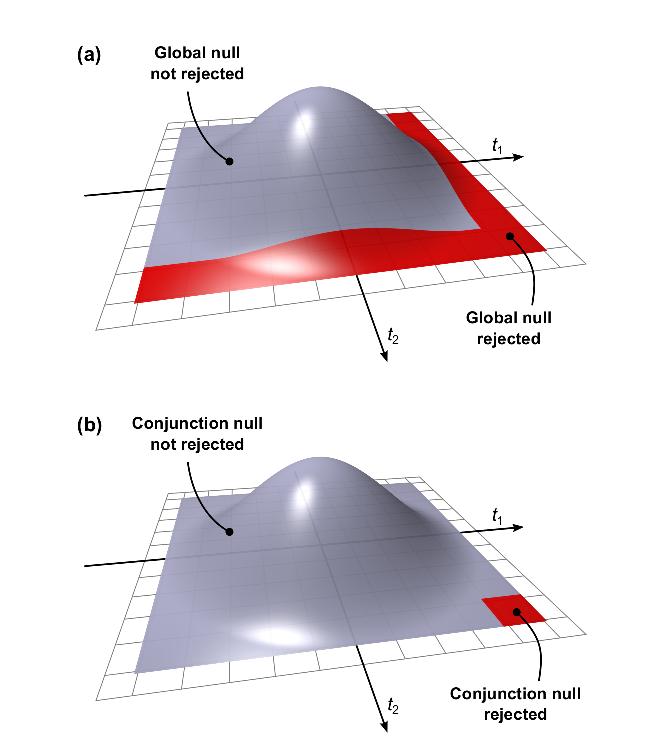
\includegraphics[scale=1.2]{images/uit_iut.eps}}
\end{center}
\caption{\emph{(a)} Rejection region of a union--intersection test (\textsc{uit}) based on two independent $t$-tests. The null is rejected if either of the partial tests has a statistic that is large enough to be qualified as significant. \emph{(b)} Rejection region of an intersection--union test (\textsc{iut}) based the same tests. The null is rejected if both the partial tests have a statistic is large enough to be qualified as significant.}
\label{fig:uit+iut}
\end{figure}

\begin{table}[!t]
\caption{Joint hypotheses tested with union--intersection and intersection--union of $K$ partial tests. In the \textsc{uit}, the null is also called \emph{global null hypothesis}, whereas in the \textsc{iut}, the null is also called \emph{conjunction null hypothesis}.}
\begin{center}
{\small
\begin{tabular}{@{}m{50mm}<{\raggedright}@{}m{30mm}<{\centering}m{30mm}<{\centering}@{}}
\toprule
{} & \textsc{uit} & \textsc{iut} \\
\midrule
Null hypothesis ($\mathcal{H}^{0}$) & \[\bigcap_{k=1}^{K} \mathcal{H}^{0}_{k}\] & \[\bigcup_{k=1}^{K} \mathcal{H}^{0}_{k}\]\\
\midrule
Alternative hypothesis ($\mathcal{H}^{1}$) & \[\bigcup_{k=1}^{K} \mathcal{H}^{1}_{k}\] & \[\bigcap_{k=1}^{K} \mathcal{H}^{1}_{k}\]\\
\bottomrule
\end{tabular}}
\end{center}
\label{tab:uit+iut}
\end{table}

Enlarging the number of tests affects \textsc{uit}s and \textsc{iut}s differently. For the \textsc{uit} with a given statistic threshold, more tests increase the chances of false positives, and correction for this multiplicity needs to be applied. In fact, it can be shown that a \textsc{uit} at a significance level $\alpha$ is equivalent to controlling the \textsc{fwer} at $\alpha$ for the same tests. In other words, a union-intersection procedure is an \textsc{fwer} procedure. For an \textsc{iut}, in contrast, the procedure does not change with more tests. The conjunction null hypothesis is \emph{composite}, consisting of different parameter settings. For the extreme case that exactly one partial null is true and $K-1$ effects are real, an \textsc{iut} is exact for any $K$; if two or more more partial nulls are true, an \textsc{iut} becomes increasingly conservative with larger $K$.

The null hypothesis of the \textsc{uit} can be rejected if the smallest $p_{k}$ is significant or, equivalently, its corresponding statistic, that is, the extremum statistic. For tests in which larger statistics provide evidence against the null hypothesis, the relevant extremum is the maximum. Conversely, for tests in which smaller statistics provide evidence  against the null, the extremum is the minimum. Clearly, if the most extreme statistic is significant, at least one partial hypothesis is rejected, therefore the global null hypothesis can be rejected without the need to continue testing the other $K-1$ partial hypotheses. The null hypothesis of the \textsc{iut} can be rejected if the largest $p_{k}$ is significant or, equivalently, its corresponding least extreme statistic. Clearly, if the least extreme statistic is significant, all partial hypotheses can be rejected, therefore the conjunction hypothesis can be rejected without the need to continue testing all other $K-1$ partial hypotheses.

In brain imaging, the term \emph{conjunction} refers to a test performed when one wants to localise regions where there is signal in all partial tests, that is, a logical \textsc{and} of all alternative hypotheses \citep{Nichols2005}, and is synonymous with the \textsc{iut}. In noting the lack of power of such a proper conjunction test, \citet{Friston2005} suggested a \emph{partial conjunction}, in which fewer than all alternatives need to intersect. Using the same notation of Table~\ref{tab:comparison}, both approaches have the same statistic, $T = \max \left(p_{k}\right)$, but the p-value of the latter can be computed as $T^{K-v+1}$, so that the test is a conjunction of at least $v$ alternative hypotheses; if $v=K$, it is an \textsc{iut}, and if $v=1$ the null is equivalent to that of a \textsc{uit} (such a test, however, is inconsistent for a \textsc{uit}; see \ref{sec:comb:consistency}). \citet{Benjamini2008} further generalised the procedure by allowing the combination of the largest p-values using any of various possible combining functions, such as those we present in Table~\ref{tab:comparison} and in \ref{sec:comb:review}.

\subsection{Closed testing}
\label{sec:comb:ctp}

In a \emph{closed testing procedure} (\textsc{ctp}), each $\mathcal{H}^0_k$ is rejected if, and only if, it is significant in its own right at a certain level $\alpha$, and if all possible sub-\textsc{jnh}s that include the same $\mathcal{H}^0_k$ and comprise some or all of the partial hypotheses (that is, subsets of the global \textsc{jnh} formed by some of the partial tests) are also rejected at $\alpha$ using a suitable test. Various such tests can be considered, including \textsc{cmv}s and \textsc{npc} (next section).

A \textsc{ctp} guarantees strong control over \textsc{fwer} \citep{Marcus1976}. To produce adjusted p-values, the original method requires that all $2^K-1$ sub-\textsc{jnh}s are tested\footnote{From the Pascal triangle: $\sum_{i=1}^K \binom{K}{i} = 2^K-1$.}, a requirement that is computationally onerous, even for a moderate number of tests, a problem aggravated by the large number of tests that are considered in an imaging experiment. There exists, however, a particular test for the sub-\textsc{jnh}s that obviates the need for such a gargantuan computational venture: the union--intersection test. In a \textsc{uit} using the extremum statistic, the most extreme of the global \textsc{jnh} that comprises all the $K$ partial tests is also the most extreme of any other sub-\textsc{jnh} that includes that particular partial hypothesis, such that the other joint subtests can be bypassed altogether. As a \textsc{uit} is also an \textsc{fwer}-controlling procedure, this raises various possibilities for correction of both \textsc{mtp-i} and \textsc{mtp-ii}. While such a shortcut can be considered for both parametric \citep{Holm1979} and non-parametric cases \citep{Westfall1993}, for the non-parametric methods using permutation, one additional feature is needed: that the joint sampling distribution of the statistic used to test each of the sub-\textsc{jnh} is the same regardless whether the null is true for all the $K$ partial tests, or just some of them. This property is called \emph{subset pivotality} \citep{Westfall1993, Westfall2008}, and it constitutes the multivariate counterpart to the univariate pivotality.

\subsection{Non-parametric combination}
\label{sec:comb:npc}

The \textsc{npc} consists of testing each of the $\mathcal{H}^0_k$ using shufflings that are performed synchronously for all $K$ partial tests. The resulting statistics for each permutation are recorded, allowing an estimate of the complete empirical null distribution to be constructed for each partial test. In a second stage, the empirical p-values for each statistic are combined, for each permutation, into a \emph{joint statistic}. As such a combined joint statistic is produced from the previous permutations, an estimate of its empirical distribution function is immediately known, and so the p-value of the unpermuted statistic, hence of the joint test, can be assessed. The method was proposed by \citet{Pesarin1990, Pesarin1992}, and independently, though less generically, by \citet{Blair1994}; a thorough description is available in \citet{Pesarin2001} and \citet{Pesarin2010}. An early application to brain imaging can be found in \citet{Hayasaka2006}, its use to combine different statistics within the same modality in \citet{Hayasaka2004}, and a summary description and practical examples are presented in \citet{Brombin2013}. The \textsc{jnh} of the combined test is that all partial null hypotheses are true, and the alternative that any is false, which is the same null of a \textsc{uit}, although the rejection region may differ widely from the example in Figure~\ref{fig:uit+iut}\emph{a}, depending on the combining function.

The only two requirements for the validity of the \textsc{npc} are that the partial test statistics have the same direction suggesting the rejection of the null hypothesis, and that they are consistent (see \ref{sec:comb:consistency}). For the combining function, it is desirable that (\textsc{i}) it is non-decreasing with respect to all its arguments (which are the p-values $p_k$, or $1-p_k$, depending on the combining function), (\textsc{ii}) that it approaches its maximum (or minimum, depending on the function) when at least one of the partial tests approaches maximum significance (that is, when at least one p-value approaches zero), and (\textsc{iii}) that for a test level $\alpha > 0$, the critical significance threshold is smaller than the function maximum value. These requirements are easily satisfied by almost all functions shown in Table~\ref{tab:comparison}, which therefore can be used as combining functions in the framework of \textsc{npc} (see \ref{sec:comb:consistency} for a discussion on the few exceptions).

One of the most remarkable features of \textsc{npc} is that the synchronised permutations implicitly account for the dependence structure among the partial tests. This means that even combining methods originally derived under an assumption of independence, such as Tippett or Fisher, can be used even when independence is untenable. In fact, modifications to these procedures to account for non-independence \citep[e.g.,][for the Fisher method]{Brown1975, Kost2002} are made redundant. As the p-values are assessed via permutations, distributional restrictions are likewise not necessary, rendering the \textsc{npc} free of most assumptions that thwart parametric methods in general. This is why \textsc{npc} methods are an alternative to \textsc{cmv} tests, as each of the response variables in a \textsc{manova} or \textsc{mancova} analysis can be seen as an univariate partial test in the context of the combination.

\subsection{Overview of combining functions}

\paragraph{Tippett} This is the oldest and probably the simplest of the combination methods, having appeared in \citet{Tippett1931}. The combined test statistic is simply the minimum p-value across all partial tests, i.e. $T_{\text{Tippett}} =$ $\min_{k} \left(p_{k}\right)$. The probability is computed as $P_{\text{Tippett}} = 1-\left(1-T_{\text{Tippett}}\right)^{K}$.

\paragraph{Fisher} This is certainly the most well known of the combination strategies. It appeared in \citet{Fisher1932} and follows from the idea of treating the joint probability as the intersection of all partial tests, which is given by their product $\prod_{k} p_{k}$. A statistic for the global hypothesis can be constructed as $T_{\text{Fisher}} =$ $-2 \sum_{k} \ln\left(p_{k}\right)$, as shown earlier in this chapter, which follows a $\chi^2$ distribution with $2k$ degrees of freedom, and from which an uniformly distributed significance level, $P_{\text{Fisher}}$, can be obtained.

\paragraph{Pearson--David} The same product suggested by Fisher, $\prod_{k} p_{k}$, was used by \citet{Pearson1933} to test equality of distributions. \citet{David1934} discussed that a similar test could be used with $\prod_{k} (1-p_{k})$ and suggested using the most extreme of these two products as the statistic, a view later shared by Pearson himself \citep{Pearson1934}. The test statistic is, therefore, given by $T_{\text{Pearson--David}}=$ $-2\min\big(\sum_{k} \ln\left(p_{k}\right),$ $\sum_{k} \ln\left(1-p_{k}\right)\big)$, which, as in the Fisher method, follows a $\chi^{2}$ distribution with $2k$ degrees of freedom, and from which the significance $P_{\text{Pearson--David}}$ can be computed.\footnote{Historical details regarding this method are recounted in \citet{Owen2009}. The authors also comment that the significance level could be doubled to account for the fact that two tests are being performed, although this is not in the original publications.}

\paragraph{Stouffer} This method appeared as a footnote in the report of the sociological study conducted among veterans of the World War \textsc{ii} by \citet{Stouffer1949}. The idea is to convert the p-values to normally-distributed $z$-scores, sum these scores, and compute a new p-value. The conversion to a normal distribution is irrespective to the distributions from which the partial p-values, $p_{k}$, may have arisen. The test statistic is given by $T_{\text{Stouffer}} =$ $\frac{1}{\sqrt{K}} \sum_{k} \Phi^{-1}\left(1-p_{k}\right)$, where $\Phi^{-1}$ is the inverse cumulative distribution function (cdf) of the normal distribution (i.e.\ the probit function). The statistic $T_{\text{Stouffer}}$ follows a normal distribution with zero mean and unit variance, from which a probability $P_{\text{Stouffer}}$ can be obtained.

\paragraph{Wilkinson} The probability of observing $r$ significant p-values at level $\alpha$ out of the $K$ tests performed can be computed using a binomial expansion as proposed by \citet{Wilkinson1951}. The statistic $T_{\text{Wilkinson}}$ is simply $r$, and the probabilty of finding no more or less than $r$ by chance is given by $P_{\text{Wilkinson}} =$ $\sum_{k=r}^{K}\binom{K}{k}\alpha^{k}(1-\alpha)^{K-k}$. If the partial p-values are sorted in ascending order, $p_{(1)} \leqslant p_{(2)} \leqslant \ldots \leqslant, p_{(K)}$, and if the significance level is defined as $\alpha=p_{(1)}$, the approach is equivalent to the Tippett method. Note that the probability does not depend on the actual probabilities for the partial tests, but only on $r$ and $\alpha$.

\paragraph{Good}  A generalisation of the Fisher method, and which assigns arbitrary, unequal positive weights $w_{k}$ for each of the p-values of the partial tests, was suggested by \citet{Good1955}. Each partial test can be weighted according to some criteria, for instance, the sample size for each of the partial test, the number of degrees of freedom, or some other desirable feature, such as ecological or internal validity \citep{Rosenthal1978}. The statistic is given by $T_{\text{Good}}=\prod_{k}p_{k}^{w_{k}}$, and its significance can be assessed as $P_{\text{Good}}=$ $\sum_{k}W_{k}T_{\text{Good}}^{1/w_{k}}$, where $W_{k}=$ $w_{k}^{K-1}$ $\left(\prod_{i=1}^{k-1}\left(w_{k}-w_{i}\right)^{-1}\right)$ $\left(\prod_{i=k+1}^{K}\left(w_{k}-w_{i}\right)^{-1}\right)$.

\paragraph{Lipt\'{a}k} Another generalised combined statistic can be produced using the inverse cdf, $F^{-1}$, of the $p_{k}$, summing the values of the statistics, and computing a new p-value for the global null using the cdf $G$ of the sum of the statistics, a method proposed by \citet{Liptak1958}. Each summand can be arbitrarily weighted, as in the Good method. In principle, any continuously increasing function with support in the interval $[0;\; 1]$ can be used for $F$, albeit a more obvious choice is the cdf of the normal distribution, which can be used as both $F$ and $G$, and which makes the approach virtually identical to the Stouffer method if all weights are 1 \citep{vanZwet1967}. In this case, the statistic for the method is given by $T_{\text{Lipt\'{a}k}} =$ $\sum_{k} w_{k}\Phi^{-1}\left(1-p_{k}\right)$, which follows a normal distribution with zero mean and variance $K$. $F$ can also be a $\chi^{2}_{\nu}$ distribution, in which case, and also when all $w_{k}=1$, $G$ is a $\chi^{2}_{K\nu}$ distribution. If $\nu=2$, the approach is equivalent to the Fisher method.

\paragraph{Lancaster} While Lipt\'{a}k method generalises combining strategies such as Fisher and Stouffer, the Lancaster method \citep{Lancaster1961} further generalises the Lipt\'{a}k approach by allowing different $F^{-1}_{k}$ for each partial test. Choices for $F^{-1}_{k}$ include, for instance, the cdf of the gamma distribution with scale parameter $\theta=2$, possibly with different shape parameters taking the place of the weights $w_{k}$ for each partial test. If the weights are all positive integers, the significances can be assessed from the cdf of a $\chi^{2}$ distribution, with degrees of freedom $\nu=2\sum_{k}w_{k}$ \citep{Berk1979}.

\paragraph{Winer} A combination strategy that resembles the Stouffer method, but uses Student's $t$ statistics, rather than $z$-scores was proposed by \citet{Winer1962}. The idea is to sum the $t$ statistics for all the $K$ partial tests, and normalising the sum so that the resulting statistic follows a standard normal distribution. The normalisation is based on the fact that the variance of the $t$ distribution can be determined from its the degrees of freedom $\nu$ as $\nu/(\nu-2)$. The statistic for this method is given by $T_{\text{Winer}}=$ $\sum_{k}t_{k}\left/\sqrt{\sum_{k}\frac{\nu_{k}}{\nu_{k}-2}}\right.$. The Winer method cannot be applied if $\nu_{k} \leqslant 2$ for any of the partial tests. Moreover, $\nu_{k}$ should not be too small for the normal approximation to be reasonably valid (e.g., $\nu_{k} \geqslant 10$). The Winer method is a particular case of the Lancaster method. {\color{orange} \emph{this all needs checking with the book!}}

\paragraph{Edgington} The probability of observing, due to chance, a value equal or smaller than the sum of the partial p-values, $T_{\text{Edgington}}=\sum_{k} p_{k}$, was proposed by \citet{Edgington1972} as a more powerful alternative to the Fisher method. This probability can be calculated as $P_{\text{Edgington}} =$ $\frac{T^K}{K!}$ when $T \leqslant 1$, where $T$ is the $T_{\text{Edgington}}$ statistic. More generally, or if $T>1$ the probability can be computed as $P_{\text{Edgington}} =$ $\sum_{j=0}^{\lfloor T \rfloor}(-1)^j \binom{K}{j}\frac{(T-j)^K}{K!}$, where $\lfloor \cdot \rfloor$ is the floor function.

\paragraph{Mudholkar--George} It is possible to use a simple logit transformation to compute a statistic that approximates a scaled version of the Student's $t$ distribution, as shown by \citet{Mudholkar1979}. The scaling can be applied to the result of the logit transformation itself, such that the statistic is computed as $T_{\text{Mudholkar--George}}$ $=$ $\frac{1}{\pi}\sqrt{\frac{3(5K+4)}{K(5K+2)}}\sum_{k} \ln\left(\frac{1-p_{k}}{p_{k}}\right)$, which follows a $t$ distribution with $5K+4$ degrees of freedom.

\paragraph{Friston (global null)} \citet{Friston1999} proposed the use of the minimum statistic, or equivalently, the maximum $p_{k}$, across the $K$ tests as a way to test the null hypothesis of no effect for all the tests. The fact that it had originally been called a ``conjunction'' caused some confusion in the literature, because the eventual rejection of the global null cannot be used to infer that the null for each of the partial tests are all rejected, as it would be in a logical conjunction \citep{Nichols2005}. The statistic for this method can be expressed in terms of the p-values for the partial tests as $T_{\text{Friston}}=$ $\max_{k} \left(p_{k}\right)$, and its significance can be assessed as $P_{\text{Friston-GN}}=T^{K}_{\text{Friston}}$. The Friston method is equivalent to the Wilkinson method if $\alpha=p_{(K)}$ and so, $r=K$.

\paragraph{Darlington--Hayes} In a discussion about pooling p-values for meta-analysis, \citet{Darlington2000} raised a number of limitations of these methods, and proposed a modification over the Stouffer method that would address some of these concerns. The modified method, called \emph{Stouffer-max}, uses as test statistic the mean of the $r$ highest $z$-scores, i.e. $T_{\text{Darlington--Hayes}} =$ $\frac{1}{r} \sum_{k=1}^{r} \Phi^{-1}\left(1-p_{(k)}\right)$, rather than the normalised sum all the $z$-scores as in the Stouffer method. When $r=1$, it is equivalent to the Tippett method, whereas when $r=K$, equivalent to the original Stouffer. Significances can be computed for intermediate values of $r$ through Monte Carlo simulation, and the authors provided tables with critical values.

\paragraph{Zaykin} This method, called \emph{truncated product method} (\textsc{tpm}) was proposed by \citet{Zaykin2002} as a way to combine features of the Fisher and Wilkinson methods. The statistic is given by $T_{\text{Zaykin}}=$ $\prod_{k=1}^{K} p_{k}^{I\left(p_{k} \leqslant \alpha\right)}$, where $I\left(\cdot\right)$ is an indicator function that evaluates as 1 if the given condition is satisfied, and 0 otherwise. In other words, the statistic is the product of only the partial p-values that are significant at the level $\alpha$, whereas in the Fisher method, all p-values are used. The significance for the combination is given by $P_{\text{Zaykin}} =$ $\sum_{k=1}^{K}\binom{K}{k}\left(1-\alpha\right)^{K-k}$ $\Big(I\left(T > \alpha^{k}\right) \alpha^{k}$ $+$ $I\left(T \leqslant \alpha^{k}\right)T\sum_{j=0}^{k-1}\frac{\left(k\ln \alpha - \ln T\right)^{j}}{j!}\Big)$, where $T$ is $T_{\text{Zaykin}}$.  If $\alpha = \min_{k}\left(p_{k}\right)$, then the approach is equivalent to the Tippett method. If $\max_{k}\left(p_{k}\right) \leqslant \alpha \leqslant 1$, the approach is equivalent to the Fisher method. Although exact, computationally the expression for $P_{\text{Zaykin}}$ is prone to over/underflows for certain combinations of large $K$ and $\alpha$, and because of this, when a global significance cannot be obtained analytically, Monte Carlo methods can be used.

\paragraph{Dudbridge--Koeleman} While the Zaykin method combines only the partial tests that are significant at the level $\alpha$, it is also possible to create a statistic that combines only the most $r$ significant tests, where $r$ is specified in advance. This method was proposed by \citet{Dudbridge2003} and called \emph{rank truncated product} (\textsc{rtp}). The main benefit of this strategy is that it depends only on a predetermined number of partial tests to be rejected, rather than on their significances, which are random quantities. The statistic is computed as $T_{\text{Dudbridge--Koeleman}}=$ $\prod_{k=1}^{r} p_{(k)}$, where $p_{(k)}$ is the p-value for the $k$-th most significant partial test. The significance can be assessed as $P_{\text{Dudbridge--Koeleman}}$ $=$ $\binom{K}{r+1}$ $\left(r+1\right)$ $\times$ $\int_0^1\left(1-t\right)^{K-r-1}$ $\left(I\left(T > t^{r}\right) t^{r} + I\left(T \leqslant t^{r}\right) T \sum_{j=0}^{r-1}\frac{\left(r\ln t - \ln T\right)^{j}}{j!}\right) \mathrm{d}t$, where $T=T_{\text{Dudbridge--Koeleman}}$. As with the Zaykin method, for certain combinations of $r$ and large $K$, the significances need to be computed through Monte Carlo methods.\footnote{A combination of the \textsc{tpm} and \textsc{rtp} has been also proposed and named \emph{rank-and-threshold truncated product} or \emph{dual truncated product} (\textsc{dtp}). The statistic is $\max\left(T_{\text{Zaykin}},T_{\text{Dudbridge--Koeleman}}\right)$ and its significance can be computed analytically or via Monte Carlo methods. See the Appendix of \citet{Dudbridge2003} for details.}

\paragraph{Nichols} Addressing logical issues regarding the original Friston method\footnote{By original we mean the method in \citet{Friston1999}. Another conjunction method had previously been proposed \citep{Price1997}, which suffered from different issues \citep{Caplan2004}.} when used for conjunctions, \citet{Nichols2005} observed that the same minimum statistic (or, equivalently, the maximum p-value) could still be used for true conjunction inference. The idea is that, if the least significant test, i.e.\ the largest $p_{k}$, is significant at $\alpha$, then all the partial tests are also significant at that level, and so, the \emph{conjunction null hypothesis}\footnote{Also called \emph{disjunction of null hypotheses} \citep{Benjamini2008}.}, i.e.\ the hypothesis that there is no effect for all or for some of the tests, can be rejected. This was the first conjunction test proposed in the neuroimaging literature\footnote{The authors had presented a the test in a poster at the \textsc{x} Annual Meeting of the Organization for Human Brain Mapping (\textsc{ohbm}), in 2004 in Budapest, Hungary \citep{Brett2004}. A similar test, with the null and alternative hypotheses reversed, had been proposed by \citet{Berger1982}.} and it does not assume independence between the partial tests.

\paragraph{Friston (conjunction null)} To address the issues that emerged about the misuse of the original test to reject the global null as a ``conjunction'', \citet{Friston2005} suggested another test, which uses the same statistic, but with the significance being computed as $P_{\text{Friston-CN}}=T^{K-u+1}_{\text{Friston}}$, where $u$ is the minimum number of partial tests that need to be rejected so that the test is a true conjunction of at least $u$ tests. When $u=K$, the approach is equivalent to the Nichols method, and when $u=1$, it is equivalent to the original Friston method. For other values of $u$, the test can be termed a \emph{partial conjunction test}.

\paragraph{Taylor--Tibshirani} If the p-values are sorted in ascending order, $p_{(1)} \leqslant p_{(2)} \leqslant \ldots \leqslant, p_{(K)}$, these ranked significances can be compared to their expectations under the global null hypothesis. Large deviations from the expected values suggest the presence of the effect among the tests. \citet{Taylor2006} suggested that a measurement of this deviation could be used to infer the overall significance of the tests. This measurement, termed \emph{tail strength} (\textsc{ts}), is defined as $T_{\text{Taylor--Tibshirani}} =$ $\frac{1}{K} \sum_{k=1}^{K} \left(1-p_{(k)}\frac{K+1}{k}\right)$. Under the assumptions that the global null is true and the tests are independent, this statistic follows a normal distribution with zero mean and a variance that can be approximated as $\sigma^2=\frac{1}{K}$ when $K \rightarrow \infty$, from which significance can be assessed. When these assumptions are not met, bootstrap inference can be used.

\paragraph{Benjamini--Heller} Recognising that sometimes a compromise between the global null and the conjunction null may be necessary, as in the Friston (conjunction null) method, \citet{Benjamini2008} proposed a generic approach in which a probability for rejecting the conjunction null in at least $u$ out of the $K$ tests is computed. In this method, the p-values are sorted in ascending order, and only those larger than $p_{(u)}$ are combined. The combination can use any of the methods that reject the global null discussed above, or others, including methods that take non-independence into account.

\paragraph{Jiang} The statistic of the Taylor--Tibshirani method has a variance that depends asymptotically only on the number of tests $K$. However, the value of the statistic can be small when effect is truly present in only a few partial tests, therefore reducing the power of the method. In an analogy with the Zaykin method, \citet{Jiang2011} proposed to compute the tail strength using only partial tests with p-values smaller than a certain level $\alpha$. The method is called \emph{truncated tail strength} (\textsc{tts}), and the statistic is computed as $T_{\text{Jiang}} =$ $\frac{1}{K} \sum_{k=1}^{K} I\left(p_{(k)}\leqslant \alpha \right)\left(1-p_{(k)}\frac{K+1}{k}\right)$. This statistic has no known analytical distribution and the authors propose computing their significance using Monte Carlo or permutation methods.

\subsection{Transformation of the statistics}

While \textsc{npc} offers flexibility in a simple and uncomplicated formulation, its implementation for brain imaging applications poses certain challenges. Because the statistics for all partial tests for all permutations need to be recorded, enormous amounts of data storage space may be necessary, a problem further aggravated when more recent, high resolution imaging methods are considered. Even if storage space were not a problem, however, the discreteness of the p-values for the partial tests becomes problematic when correcting for multiple testing, because with thousands of tests in an image, ties are very likely to occur among the p-values, further causing ties among the combined statistics. If too many tests across an image share the same most extreme statistic, correction for the \textsc{mtp-i}, while still valid, becomes less powerful \citep{Westfall1993, Pantazis2005}. The most obvious workaround --- run an ever larger number of permutations to break the ties --- may not be possible for small sample sizes, or when possible, requires correspondingly larger data storage.

However, another possible approach can be considered after examining the two requirements for the partial tests, and also the desirable properties (\textsc{i})--(\textsc{iii}) of the combining functions, all listed earlier. These requirements and properties are quite mild, and if the sample size is reasonably large and the test statistics homogeneous, i.e., they share the same asymptotic permutation distribution, a \emph{direct combination} based not on the p-values, but on the statistics themselves, such as their sum, can be considered \citep[page 131]{Pesarin2010}. Sums of statistics are indeed present in combining functions such as of Stouffer, Lancaster, Winer, and Darlington--Hayes, but not others listed in Table~\ref{tab:comparison} and \ref{sec:comb:review}. In order to use these other combining functions, most of them based on p-values for the partial tests, and under the same premises, the statistics need to be transformed to quantities that behave as p-values. In the parametric case, these would be the parametric p-values, computed from the parametric cumulative distribution function (cdf) of the test statistic. If the parametric assumptions are all met for the partial tests, their respective parametric p-values are all valid and exact; if the assumptions are not met, these values are no longer appropriate for inference on the partial tests, but may still be valid for \textsc{npc}, for satisfying all requirements and desirable properties of the combining functions. As they are not guaranteed to be appropriate for inference on the partial tests, to avoid confusion, we call these parametric p-values ``u-values''.

Another reason for not treating u-values as valid p-values is that they do not necessarily need to be obtained via an assumed, parametric cumulative distribution function for the statistics of the partial tests. If appropriate, other transformations applied to the statistics for the partial tests can be considered; whichever is more accurate to yield values in the interval $[0;1]$ can be used. The interpretation of a u-value should not be that of a probability, but merely of a monotonic, deterministic transformation of the statistic of a partial test, so that it conforms to the needs of the combining functions.

Transformation of the statistic to produce quantities that can be used in place of the non-parametric p-values effectively simplifies the \textsc{npc} algorithm, greatly reducing the data storage requirements and computational overhead, and avoiding the losses in power induced by the discreteness of p-values. This simplification is shown in Figure~\ref{fig:flowchart}, alongside the original \textsc{npc} algorithm.

\begin{figure}[p]
%\thisfloatpagestyle{empty}
\begin{center}
\centerline{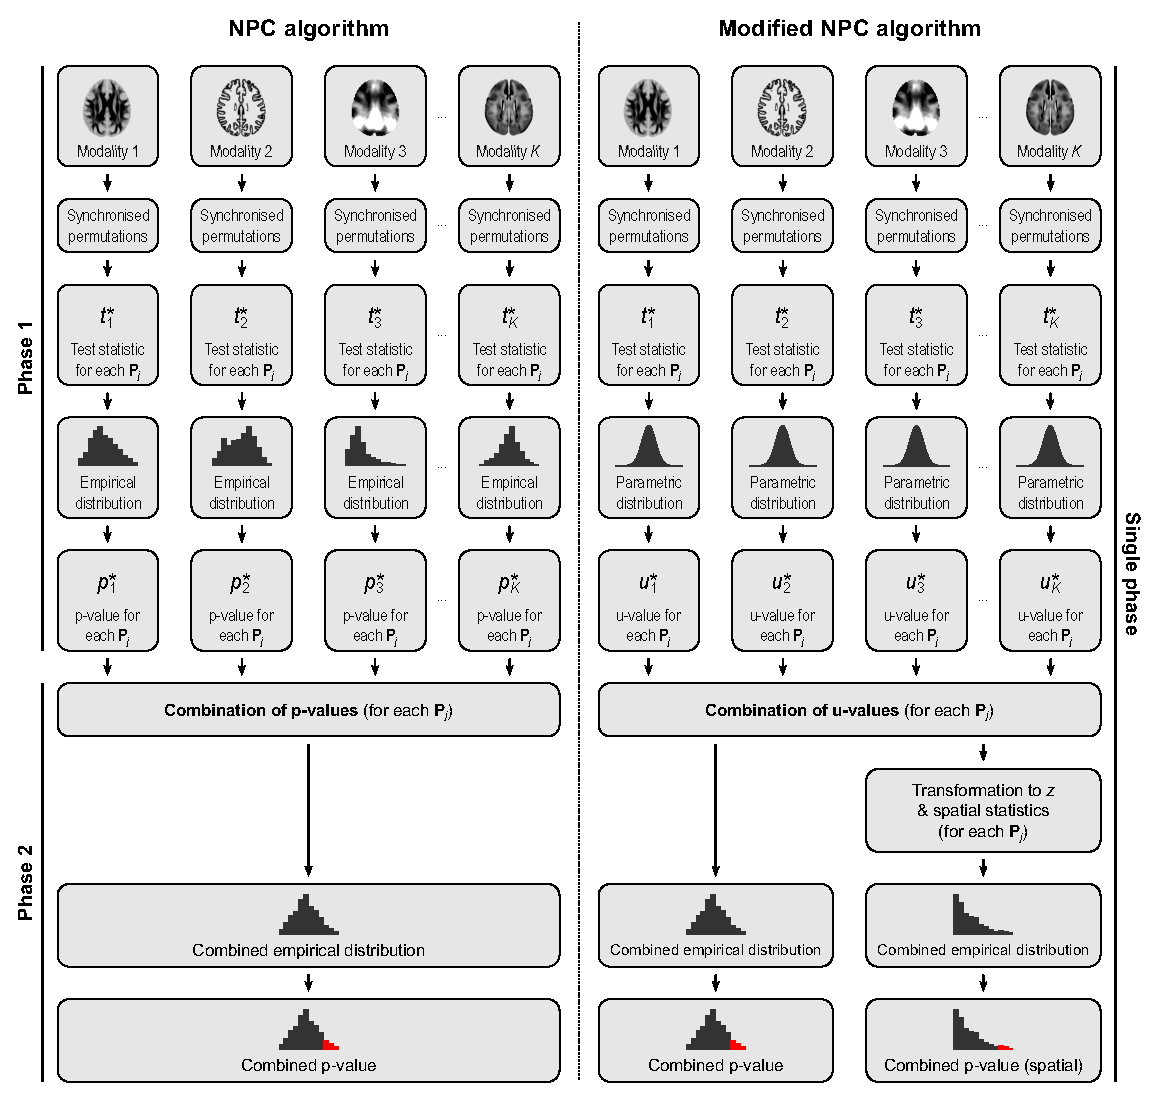
\includegraphics[scale=.8]{images/flowchart.eps}}
\end{center}
\caption{The original \textsc{npc} algorithm combines non-parametric p-values and, for imaging applications, requires substantial amount of data storage space. Two modifications simplify the procedures: (\textsc{i}) the statistic $t_k$ for each partial test $k$ is transformed into a related quantity $u_k$ that has a behaviour similar to the p-values, and (\textsc{ii}) the combined statistic is transformed to a variable that follows approximately a normal distribution, so that spatial statistics (such as cluster extent, cluster mass, and \textsc{tfce}) can be computed as usual. The first simplification allows the procedure to run in a single phase, without the need to retrieve data for the empirical distribution of the partial tests.}
\label{fig:flowchart}
\end{figure}

Regardless of the above transformation, the distribution of the combined statistic, $T$, may vary greatly depending on the combining function, and it is always assessed non-parametrically, via permutations. Different distributions for different combining functions can, however, pose practical difficulties when computing spatial statistics such as cluster extent, cluster mass, and even threshold-free cluster enhancement \citep[\textsc{tfce},][]{Smith2009}. Consider for instance the threshold used to define clusters: prescribed values such as 2.3 or 3.1 \citep{Woo2014} relate to the normal distribution and are not necessarily sensible choices for combining functions such as Tippett or Fisher. Moreover, for some combining functions, such as Tippett and Edgington, smaller values for the statistic are evidence towards the rejection of the null, as opposed to larger as with most of the others. To address these practical issues, a monotonic transformation can be applied to the combined statistic, so that its behaviour becomes more similar to, for instance, the $z$-statistic \citep{Efron2004}. This can be done again by resorting to the asymptotic behaviour of the tests: the combined statistic is converted to a parametric p-value (the formulas are summarised in Table~\ref{tab:comparison}), which, although not valid for inference unless certain assumptions are met, particularly with respect to the independence among the partial tests, are useful to transform, at each permutation, the combined statistic to the $z$-statistic, which can then be used for inference using cluster extent, mass, or \textsc{tfce}.

\subsection{Consistency of combined tests}
\label{sec:comb:consistency}

A hypothesis test is said to be \emph{consistent} if, for a fixed test level, its power goes to unity as the sample size increases to infinity. The use of a non-consistent combining function to form an \textsc{npc} test is problematic, as the rejection region may not be reached even if the p-value for one or more of the partial tests approach zero, thus violating the second of the three desirable properties of the combining functions, presented in Section~\ref{sec:comb:npc}.

Among the functions shown in Table~\ref{tab:comparison}, the notable non-consistent combining functions are the Edgington and Wilkinson (see \ref{sec:comb:review}). Also, it should be noted that functions that define conjunctions (\textsc{iut}), such as those based on $\max\left(p_k\right)$, are likewise not consistent in the context of \textsc{npc}, as the latter serves to test the global null hypothesis. Figure~\ref{fig:inconsistent} shows rejection regions for some inconsistent combining functions, and variants, similarly as for the (consistent) shown in Figure~\ref{fig:rejection}.

\begin{figure}[p]
\begin{center}
\centerline{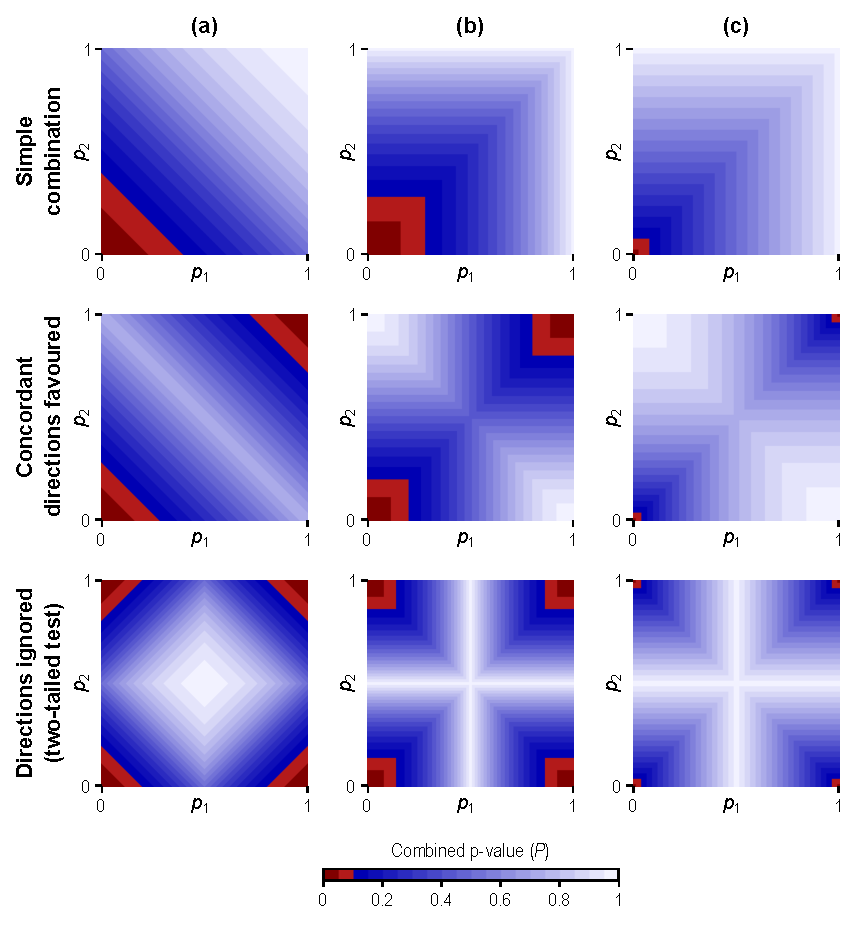
\includegraphics[scale=.8]{images/inconsistent.eps}}
\end{center}
\caption{Examples of inconsistent combining functions for testing the global null hypothesis: \emph{(a)} Addition of p-values for the partial tests \citep{Edgington1972}; \emph{(b)} Maximum of p-values for the partial tests, with the p-value computed as $T^K$ \citep{Friston1999, Friston2005}; \emph{(c)} Maximum of p-values for the partial tests, but with the p-value computed as $T$ \citep{Nichols2005}. While the last is not appropriate for testing the global null, it is appropriate for the conjunction null.}
\label{fig:inconsistent}
\end{figure}

\subsection{Admissibility of combined tests}
\label{sec:comb:admissibility}

A combined hypothesis test is said to be \emph{admissible} if there exists no other test that, at the same significance level, without being less powerful to all possible alternative hypotheses, is more powerful to at least one alternative \citep{Lehmann2005}. This can be stated in terms of either of two sufficient conditions for admissibility: (\textsc{i}) that rejection of the null for a given p-value implies the rejection of the null for all other p-values smaller or equal than that, or (\textsc{ii}) that the rejection region is convex in the space of the test statistic.

Combinations that favour tests with concordant directions (Section~\ref{sec:comb:directed}), if used with of non-directional partial tests, create tests that are inadmissible, that is, tests that are not optimal in the sense that there exist other tests that, without being less powerful to some true alternative hypotheses, are more powerful to at least one true alternative. Inadmissibility implies that the test cannot be used, as certain combinations of partial tests lead to nonsensical results, such as rejecting the \textsc{jnh} for some partial p-values, and failing to reject for some p-values that are even smaller. Figure~\ref{fig:inadmissible} shows rejection regions of inadmissible versions of the combining functions considered in Figures~\ref{fig:rejection} and \ref{fig:inconsistent}; clearly none of the two conditions above are satisfied. The particular combining function shown in Equation~\ref{eqn:pearson-david} was suggested by \citet{Pearson1933} and used by \citet{David1934}, but after a paper by \citet{Birnbaum1954}, it was for decades thought to be inadmissible. However, it is in fact admissible \citep{Owen2009}.

\begin{figure}[!p]
\begin{center}
\centerline{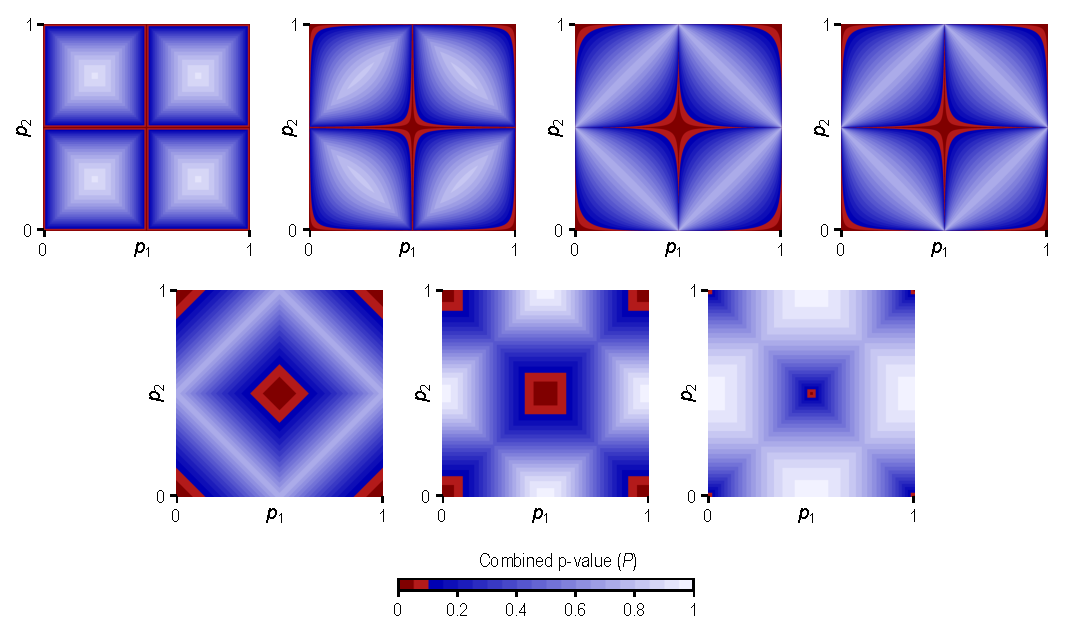
\includegraphics[scale=.8]{images/inadmissible.eps}}
\end{center}
\caption{\emph{Upper row:} Inadmissible versions of the four consistent combining functions shown in Figure~\ref{fig:rejection} (in the same order). \emph{Lower row:} Inadmissible versions of the three inconsistent combining functions shown in Figure~\ref{fig:inconsistent} (in the same order). These inadmissible functions arise if one attempts to favour alternatives with the same sign while performing two-tailed partial tests.}
\label{fig:inadmissible}
\end{figure}

Admissibility is important in that it allows, for more than just two partial tests, combined tests that favour alternative hypotheses with the same direction. Other possibilities favouring alternatives with common direction, such as multiplying together the partial test statistics to produce a combined statistic, work for two partial tests only \citep{Hayasaka2006}.

\subsection{Directed, non-directed, and concordant hypotheses}
\label{sec:comb:directed}

When the partial hypotheses are one-sided, i.e., $\mathcal{H}^{0}_{k} : \mathbf{C}'\boldsymbol{\beta}_{k} > 0$ or $\mathcal{H}^{0}_{k} : \mathbf{C}'\boldsymbol{\beta}_{k} < 0$, and all have the same direction (either), the methods presented thus far can be used as described. If not all have the same direction, a subset of the tests can be scaled by $-1$ to ensure a common direction for all.

If the direction is not relevant, but the concordance of signs towards one of them (either) is, a new combining test can be constructed using one-sided p-values, $p_k$, and another using $1-p_k$, then taking the best of these two results after correcting for the fact that two tests were performed. For example, for the Fisher method, we would have:

\begin{equation}
T = \max\left(-2\sum_{k=1}^{K} \ln\left(p_{k}\right),-2\sum_{k=1}^{K} \ln\left(1-p_{k}\right)\right)
\label{eqn:pearson-david}
\end{equation}

\noindent
where $T$ is the combined test statistic, with its p-value, $P$, assessed via permutations.

If direction or concordance of the signs are not relevant, two-sided (non-directed) tests and p-values can be used before combining, that is, ignoring the sign of the test statistic for the partial tests, or using a statistic that is non-directional (e.g., with $F$-tests for the partial hypotheses). It worth mentioning, however, that it is not appropriate to simultaneously ignore directions of the partial tests \emph{and} use a combination that favours concordant signs. Such a test would lack meaning and would be inadmissible, with examples shown in \ref{sec:comb:admissibility}. 

Rejection regions for these three cases, for four different combining functions, are shown in Figure~\ref{fig:rejection}, as functions of the partial p-values, for $K=2$ partial tests.

\begin{figure}[p]
\begin{center}
\centerline{\includegraphics[scale=.8]{images/rejection.eps}}
\end{center}
\caption{
\emph{Upper row:} Rejection regions for the combination of two partial tests using four different combining functions, and with the p-values assessed parametrically (Table~\ref{tab:comparison}). The regions are shown as function of the p-values of the partial tests ($p_k$).
\emph{Middle row:} Rejection regions for the same functions with the modification to favour alternative hypotheses with concordant directions.
\emph{Lower row:} Rejection regions for the same functions with the modification to ignore the direction altogether, that is, for two-tailed partial tests.}
\label{fig:rejection}
\end{figure}

\subsection{The method of Tippett}

From the various combining functions listed in Table~\ref{tab:comparison}, consider the combining function of \citet{Tippett1931}, that has statistic $T = \min {p_{k}}$ and, when all partial tests are independent, a p-value $P = 1-(1-T)^K$. This test has interesting properties that render it particularly attractive for imaging:

\begin{itemize}[leftmargin=*]
\item[--] It defines a \textsc{uit} test: If the minimum p-value remains significant when all tests are considered, clearly the global null hypothesis can be rejected.
\item[--] It controls the \textsc{fwer}: Controlling the error rate of a \textsc{uit} is equivalent to an \textsc{fwer}-controlling procedure over the partial tests.
\item[--] If the partial tests are independent, it defines an exact \textsc{fwer} threshold: The function is closely related to \citet{Sidak1967} correction: set $P=\alpha^{\text{\textsc{fwer}}}$, then $T^{\text{\textsc{fwer}}}=1-(1-\alpha^{\text{\textsc{fwer}}})^{\frac{1}{K}}$; one can retain only the partial p-values that satisfy $p_k \leqslant T^{\text{\textsc{fwer}}}$. Adjusted p-values can be obtained similarly through the \v{S}id\'{a}k procedure, that is $p_k^\textsc{fwer}=1-(1-p_k)^{\frac{1}{K}}$.
\item[--] If the partial tests are not independent, it still defines an \textsc{fwer} threshold and adjusted p-values: As a \textsc{uit}, the Tippett function can be used in a closed testing procedure. Further, it is \emph{the} function that makes \textsc{ctp} with large $K$ feasible in practice; adjusted p-values are obtained with the distribution of the minimum p-value (or of the extremum statistic).
\item[--] Because it subsumes correction using the extremum statistic that is already in use in imaging to account for \textsc{mtp-i}, the correction for the \textsc{mtp-ii} can be done by pooling the maximum statistics across both space and the set of partial tests. This allows algorithmic advantages that we exploit in the proposed implementation shown in \ref{sec:comb:implementation}.
\item[--] It can be used as the combining function with \textsc{npc}, thus providing a common procedure for correction and for combination of p-values.
\item[--] It is fast to compute: Taking the extremum statistic or minimum p-value is trivial compared to other functions that require cumulative sums or products, multiple parameters, integrations, or that depend on Monte Carlo simulations.
\end{itemize}

While the Tippett function is advantageous for all these reasons, note that, even when other combining functions are used for \textsc{npc}, the extremal statistic (equivalent to the Tippett combining function) is also used for the \textsc{mtp-i} to control \textsc{fwer} over space.

\subsection{A unified procedure}

Armed with these concepts, and with the modifications to the original \textsc{npc} algorithm, we are positioned to tackle the various problems identified in the \href{sec:comb:intro}{Introduction}:

\paragraph{Combination of multiple modalities} With $K$ modalities, all in register and with the same spatial resolution, each is tested separately, using synchronised permutations, and their statistics converted to u-values for each shuffling. These are are combined using a suitable combining function, such as one from those shown in Table~\ref{tab:comparison}. The p-values for the combined statistic are produced using the same set of permutations used to assess each test separately. This is the modified \textsc{npc} algorithm that we propose, shown in Figure~\ref{fig:flowchart}.

\paragraph{Correction for multiple modalities} With $K$ modalities, which are not necessarily in register, nor with the same resolution, nor of the same type (e.g., some from volumetric, some from surface representations of the brain), or which may not necessarily be all related to imaging (e.g., some imaging and some non-imaging data), each is tested separately using a suitable test statistic. The permutation distribution of the extremum statistic across \emph{all} tests is produced and used to compute \textsc{fwer}-adjusted p-values that simultaneously address the \textsc{mtp-i} and \textsc{mtp-ii}.

\paragraph{Correction for multiple designs and contrasts} Each pair of contrasts defined by $\left(\mathbf{C}, \mathbf{D}\right)$ allows the corresponding design matrix to be partitioned into effects of interest and nuisance effects \citep[][Appendix A]{Winkler2014}, and also the redefinition of the response variables (Section \ref{sec:comb:notation}). Thus, multiple designs and their respective contrasts can be tested separately. Differently than for the correction for multiple modalities, however, with different contrasts, their respective statistics may possess different asymptotic behaviour (due to, e.g., the contrasts having different ranks, or the designs having different degrees of freedom), thus precluding the use of the distribution of the extremum statistic. When known, the asymptotic behaviour can be used to convert these statistics --- univariate or multivariate --- to a $z$-statistic. The distribution of the maximum across the results of the various designs and contrasts can then be computed and used for correction.

\paragraph{Correction for multiple modalities, designs and contrasts} Following the same principles, it is also possible to account for the multiplicity of input modalities, each tested with their respective design and set of contrasts, or each tested versus all designs and contrasts. Each test is applied separately, statistics converted to a $z$-statistic based on their asymptotic behaviour, and the distribution of the extremum used to obtain adjusted p-values for all in a \textsc{ctp} using a \textsc{uit}. It is not necessary that all are in register, neither that all use the same kind of image representation of the brain (i.e., volume or surface), nor that they are even all (or any) imaging-related, and can therefore include clinical or behavioural, biomarkers, and other types of data.

\paragraph{Conjunctions} An \textsc{iut} can be assessed through permutations simply by computing $\max \left(p_{k}\right)$, which is, in its own right, the p-value of the \textsc{iut}, such that there is no need for transformation into u-values for the assessment of the combined statistic. In the context of imaging, such conjunctions can be used with statistics at every voxel (or vertex or face), thus allowing also certain spatial statistics such as \textsc{tfce}.

\vspace{10pt}

Since combinations and conjunctions are performed at each individual image point, it is necessary that all images have been registered to the same common space and possess similar spatial resolution \citep{Lazar2002}. This can be accomplished through intra-subject and inter-subject registration and resampling. By contrast, correction for the multiplicity of tests uses the maximum statistic across such tests, thus not requiring that the tests match on space, or even that they are all related to imaging. However, they explicitly require pivotal statistics \citep[for pivotality in this context, see][]{Winkler2014}, so that the extreme is taken from statistics that share the same sampling distribution. The statistics used with \textsc{cmv} and \textsc{npc} are all pivotal and therefore can be used. Spatial statistics, however, lack this property and require similar search volumes and resolutions, even for correction. Moreover, by including information from neighbouring voxels, such as using spatial smoothing or spatial statistics like \textsc{tfce} \citep{Smith2009}, subset pivotality is lost, meaning that strong control of \textsc{fwer} cannot be guaranteed. In practice, though, the power gained by pooling information over space is essential. In the \ref{sec:comb:implementation} we provide an algorithm that generically implements the combination and correction methods presented.

%\subsection{Implementation}
\label{sec:comb:implementation}

A unified algorithm for combination and correction that is amenable for use with imaging applications is shown below. It has many similarities with the \texttt{randomise} algorithm \citep{Winkler2014}, with various modifications to accommodate combination and correction. The p-values adjusted for the multiplicity of tests are computed using the distribution of the extremum statistic, which can be collapsed across modalities and/or designs and contrasts for each case, rendering the algorithm simpler. The notation below is slightly different than that used throughout the paper. The inputs are:

\begin{itemize}[leftmargin=*]
\item[--] $\mathbf{Y}$: The input data for each of the $K$ modalities and image points. Each column vector of $N$ observations for the $k$-th modality is accessed as $\mathbf{Y}[k,\mathbf{v}]$, where $\mathbf{v}=[x, y, z]$ is used to specify the point position in space; this is so without loss of generality for non-imaging data.
\item[--] $\mathcal{X}$:  The set of design matrices $\mathbf{X}$.
\item[--] $\{\mathcal{C}_\mathbf{X}\}$: The set of sets of contrasts for each design matrix $\mathbf{X}$. Each element of each subset is a pair of multivariate contrasts $(\mathbf{C},\mathbf{D})$. This definition allows each design to be tested with multiple such pairs of contrasts, and allows various designs to be tested with the same input data.
\item[--] $\mathbf{B}$: Definition of multi-level exchangeability blocks, used to define valid shufflings that respect the data structure \citep{Winkler2015}.
\item[--] $\mathbf{V}$: Definition of the variance groups, useful to compute statistics that are robust to heteroscedasticity.
\item[--] \textsc{ee}, \textsc{ise}: Boolean flags (true/false) indicating whether errors can be treated as exchangeable (\textsc{ee}), allowing permutations, independent and symmetric (\textsc{ise}), allowing sign-flippings, or both.
\item[--] $J$: Number of permutations to be performed.
\item[--] \textsc{npcmod}, \textsc{npccon}: Boolean indicating whether combination should be performed respectively across modalities, across designs and contrasts, or both.
\item[--] \textsc{fwemod}, \textsc{fwecon}: Boolean indicating whether familywise error rate correction should be performed respectively across modalities, across designs and contrasts, or both.
\end{itemize}

The output of interest is the p-value. For simplicity, as shown, the output is always \textsc{fwer}-adjusted across the image points indexed by $\mathbf{v}$, and for the non-combined, further adjusted based on the contrasts and modalities; these are shown in the algorithm topped by a tilde, that is, as ``$\tilde{\text{p}}$-value'', as opposed to simply ``p-value''. Also for simplicity, p-values for combination of modalities are not shown adjusted for multiple contrasts, nor vice-versa. These can also be obtained following the same logic used for the \textsc{fwer}-adjustment of the non-combined statistics. Uncorrected p-values, useful for correction using false discovery rate \citep[\textsc{fdr},][]{Benjamini1995} can be obtained with trivial modifications. 

\vspace{4mm}
\singlespacing
\noindent Algorithm 1: Unified algorithm. See the main text for details.\\
\HRule
\vspace{1mm}
\algrenewcommand\algorithmicindent{1em}
{\small
\begin{algorithmic}[1]
\Require $\mathbf{Y}, \mathcal{X}, \{\mathcal{C}_\mathbf{X}\}, \mathbf{B}, \mathbf{V}, \textsc{ee}, \textsc{ise}, J, \textsc{npcmod}, \textsc{npccon}, \textsc{fwemod}, \textsc{fwecon}$.
\State $\mathcal{P} \leftarrow \text{\textsf{sync\_perms}}(\mathcal{X}, \{\mathcal{C}_\mathbf{X}\}, \mathbf{B}, \textsc{ee}, \textsc{ise},J-1)$
\Comment{Define the permutation set.}
\State $\mathcal{P} \leftarrow \{\mathbf{I}, \mathcal{P}\}$
\Comment{Ensure first permutation is no permutation.}
\For{$j = 1, \ldots , J$}
\Comment{For each shuffling.}
\State $c \leftarrow 1$
\Comment{Counter for the number of designs and contrasts.}
\ForAll{$\mathbf{X} \in \mathcal{X}$}
\Comment{For each design matrix.}
\ForAll{$(\mathbf{C},\mathbf{D}) \in \mathcal{C}_\mathbf{X}$}
\Comment{For each pair of contrasts.}
\State $\mathbf{Y} \leftarrow \mathbf{Y}\mathbf{D}$
\Comment{Redefine the data, discard $\mathbf{D}$.}
%\State $\mathbf{X}, \mathbf{Z}, \mathbf{C} \leftarrow \text{\textsf{partition}}(\mathbf{X}, \mathbf{C})$
%\Comment{Partition the model, redefine $\mathbf{C}$.}
%\State $\mathbf{X} \leftarrow [\mathbf{X}\;\mathbf{Z}]$
%\Comment{For simplicity, concatenate the partitions.}
\State $\mathbf{X^{*}} \leftarrow \mathbf{P}_{j}\mathbf{X}$
\Comment{Shuffle the model.}
\ForAll{$k \in \{1, \ldots , K\}$}
\Comment{For each partial test.}
\ForAll{$\mathbf{v}$}
\Comment{For each image point.}
\State $\boldsymbol{\hat{\beta}} \leftarrow (\mathbf{X^{*}})^{+}\mathbf{Y}[k,\mathbf{v}]$
\Comment{Estimated regression coefficients.}
\State $\mathbf{\hat{E}} \leftarrow \mathbf{Y}[k,\mathbf{v}] - \mathbf{X^{*}}\boldsymbol{\hat{\beta}}$
\Comment{Estimation residuals.}
\State $\mathbf{G} \leftarrow \text{\textsf{pivotal}}(\mathbf{X^{*}},\boldsymbol{\hat{\beta}},\hat{\boldsymbol{\epsilon}},\mathbf{C},\mathbf{V})$
\Comment{Test statistic.}
\State $\mathbf{U}[j,k,c,\mathbf{v}] \leftarrow \text{\textsf{transform}}(\mathbf{G})$
\Comment{Transform to u-value.}
\If {$j = 1$}
\Comment{In the first permutation (no permutation).}
\State $\mathbf{U}_0[k,c,\mathbf{v}] \leftarrow \mathbf{U}[1,k,c,\mathbf{v}]$
\Comment{Keep the unpermuted u-value.}
\EndIf
\EndFor
\State $\mathbf{U}_{\text{e}}[j,k,c] \leftarrow \text{\textsf{extremum}}(\mathbf{U}[j,k,c,\cdot])$
\Comment{Extremum across space.}
\EndFor
\State $c \leftarrow c + 1$
\Comment{Increment counter for the number of designs and contrasts.}
\EndFor
\EndFor
\State $C \leftarrow c$
\Comment{Keep the total number of designs and contrasts for later use.}
\If {\textsc{npcmod} $\wedge$ \textlnot\ \textsc{npccon}}
\Comment{Combine modalities only.}
\ForAll{$c \in \{1, \ldots, C\}$}
\Comment{For each design/contrast.}
\ForAll{$\mathbf{v}$}
\Comment{For each image point.}
\State $\mathbf{T}[c,\mathbf{v}] \leftarrow \text{\textsf{combine}}(\mathbf{U}[j,\cdot,c,\mathbf{v}])$
\Comment{Combined statistic.}
\EndFor
\State $\mathbf{T}_{\text{e}}[j,c] \leftarrow \text{\textsf{extremum}}(\mathbf{T}[c,\cdot])$
\Comment{Distribution of the extrema across tests.}
\EndFor
\ElsIf {\textsc{npccon} $\wedge$ \textlnot\ \textsc{npcmod}}
\Comment{Combine designs/contrasts only.}
\ForAll{$k \in \{1, \ldots, K\}$}
\Comment{For each design/contrast.}
\ForAll{$\mathbf{v}$}
\Comment{For each image point.}
\State $\mathbf{T}[k,\mathbf{v}] \leftarrow \text{\textsf{combine}}(\mathbf{U}[j,k,\cdot,\mathbf{v}])$
\Comment{Combined statistic.}
\EndFor
\State $\mathbf{T}_{\text{e}}[j,k] \leftarrow \text{\textsf{extremum}}(\mathbf{T}[k,\cdot])$
\Comment{Distribution of the extrema across tests.}
\EndFor
\ElsIf {\textsc{npcmod} $\wedge$ \textsc{npccon}}
\Comment{Combine modalities \& designs/contrasts.}
\ForAll{$\mathbf{v}$}
\Comment{For each image point.}
\State $\mathbf{T}[\mathbf{v}] \leftarrow \text{\textsf{combine}}(\mathbf{U}[j,\cdot,\cdot,\mathbf{v}])$
\Comment{Combined statistic.}
\EndFor
\State $\mathbf{T}_{\text{e}}[j] \leftarrow \text{\textsf{extremum}}(\mathbf{T}[\cdot])$
\Comment{Distribution of the extrema across tests.}
\EndIf
\If {$j = 1$}
\Comment{In the first permutation (no permutation).}
\State $\mathbf{T}_0 \leftarrow \mathbf{T}$
\Comment{Keep the unpermuted combined statistic.}
\EndIf
\EndFor
\If {\textsc{npcmod} $\wedge$ \textlnot\ \textsc{npccon}}
\Comment{Combine modalities only.}
\ForAll{$c \in \{1, \ldots, C\}$}
\Comment{For each design/contrast.}
\ForAll{$\mathbf{v}$}
\Comment{For each image point.}
\State{p-value$[c,\mathbf{v}] \leftarrow \text{\textsf{data\_pval}}(\mathbf{T}_0[c,\mathbf{v}],\mathbf{T}_{\text{e}}[\cdot,c])$}
\Comment{Combined p-value.}
\EndFor
\EndFor
\ElsIf {\textsc{npccon} $\wedge$ \textlnot\ \textsc{npcmod}}
\Comment{Combine designs/contrasts only.}
\ForAll{$k \in \{1, \ldots, K\}$}
\Comment{For each design/contrast.}
\ForAll{$\mathbf{v}$}
\Comment{For each image point.}
\State{p-value$[k,\mathbf{v}] \leftarrow \text{\textsf{data\_pval}}(\mathbf{T}_0[k,\mathbf{v}],\mathbf{T}_{\text{e}}[\cdot,k])$}
\Comment{Combined p-value.}
\EndFor
\EndFor
\ElsIf {\textsc{npcmod} $\wedge$ \textsc{npccon}}
\Comment{Combine modalities \& designs/contrasts.}
\ForAll{$\mathbf{v}$}
\Comment{For each image point.}
\State{p-value$[\mathbf{v}] \leftarrow \text{\textsf{data\_pval}}(\mathbf{T}_0[\mathbf{v}],\mathbf{T}_{\text{e}}[\cdot])$}
\Comment{Combined p-value.}
\EndFor
\EndIf
\If {\textsc{fwemod} $\wedge$ \textlnot\ \textsc{fwecon}}
\Comment{Correct over modalities only.}
\ForAll{$c \in \{1, \ldots, C\}$}
\Comment{For each design/contrast.}
\ForAll{$j \in \{1, \ldots, J\}$}
\Comment{For each shuffling.}
\State $\mathbf{U}'_{\text{e}}[j,c] \leftarrow \text{\textsf{extremum}}(\mathbf{U}_{\text{e}}[j,\cdot,c])$
\Comment{Distribution of the extrema.}
\EndFor
\ForAll{$k \in \{1, \ldots, K\}$}
\Comment{For each modality.}
\ForAll{$\mathbf{v}$}
\Comment{For each image point.}
\State{$\tilde{\text{p}}$-value$[k,c,\mathbf{v}] \leftarrow \text{\textsf{data\_pval}}(\mathbf{U}_0[k,c,\mathbf{v}],\mathbf{U}'_{\text{e}}[\cdot,c])$}
\Comment{Adjusted p-value.}
\EndFor
\EndFor
\EndFor
\ElsIf {\textsc{fwecon} $\wedge$ \textlnot\ \textsc{fwemod}}
\Comment{Correct over designs/contrasts only.}
\ForAll{$k \in \{1, \ldots, K\}$}
\Comment{For each modality.}
\ForAll{$j \in \{1, \ldots, J\}$}
\Comment{For each shuffling.}
\State $\mathbf{U}'_{\text{e}}[j,k] \leftarrow \text{\textsf{extremum}}(\mathbf{U}_{\text{e}}[j,k,\cdot])$
\Comment{Distribution of the extrema.}
\EndFor
\ForAll{$c \in \{1, \ldots, C\}$}
\Comment{For each design/contrast.}
\ForAll{$\mathbf{v}$}
\Comment{For each image point.}
\State{$\tilde{\text{p}}$-value$[k,c,\mathbf{v}] \leftarrow \text{\textsf{data\_pval}}(\mathbf{U}_0[k,c,\mathbf{v}],\mathbf{U}'_{\text{e}}[\cdot,k])$}
\Comment{Adjusted p-value.}
\EndFor
\EndFor
\EndFor
\ElsIf {\textsc{fwemod} $\wedge$ \textsc{fwecon}}
\Comment{Correct over modalities \& des./contr.}
\ForAll{$j \in \{1, \ldots, J\}$}
\Comment{For each shuffling.}
\State $\mathbf{U}'_{\text{e}}[j] \leftarrow \text{\textsf{extremum}}(\mathbf{U}_{\text{e}}[j,\cdot,\cdot])$
\Comment{Distribution of the extrema.}
\EndFor
\ForAll{$k \in \{1, \ldots, K\}$}
\Comment{For each modality.}
\ForAll{$c \in \{1, \ldots, C\}$}
\Comment{For each design/contrast.}
\ForAll{$\mathbf{v}$}
\Comment{For each image point.}
\State{$\tilde{\text{p}}$-value$[k,c,\mathbf{v}] \leftarrow \text{\textsf{data\_pval}}(\mathbf{U}_0[k,c,\mathbf{v}],\mathbf{U}'_{\text{e}}[\cdot])$}
\Comment{Adjusted p-value.}
\EndFor
\EndFor
\EndFor
\EndIf
\end{algorithmic}}
\noindent
\HRule\\
% \doublespacing
\setstretch{\lspac}
\vspace{0mm}

Within the algorithm, the functions are:

\begin{itemize}[leftmargin=*]
\item[--] \emph{sync\_perms}: This function produces a set $\mathcal{P}$ of permutation and/or sign flipping matrices that can be performed sychronously to test a joint null hypotheses about the input data. The synchronisation is always necessary to allow combination/correction over modalities, and it may also be necessary across multiple designs and/or contrasts if these are to be combined/corrected as well. If synchronisation is not necessary for designs and/or contrasts, the algorithm can be modified so that $\mathcal{P}$ can be defined inside the for-loops that iterate over designs and contrasts.
\item[--] \emph{transform}: This converts the test statistic into a u-value, thus rendering the \textsc{npc} method feasible for imaging applications. If no combination is to be performed, the algorithm can be modified to skip this step and work directly with the test statistic.
\item[--] \emph{extremum}: For statistics in which larger values are evidence against the null hypothesis, this function takes the maximum. For statistics in which smaller values are indication against the null, this takes the minimum. In either case, it is always the most extreme towards evidence favouring the alternative. This function effectively implements a \textsc{ctp} using an \textsc{iut}.
\item[--] \emph{combine}: This combines the inputs (p- or u-values) into a new, combined statistic. Any of the combining functions from Table~\ref{tab:comparison} can be considered. For the method of Tippett, \emph{combine} and \emph{extremum} are the same.
\item[--] \emph{data\_pval}: This function produces a p-value based on a set of empirical values for the test statistic after shuffling. This works by computing the fraction of the test statistics after shuffling that is larger or equal than the unpermuted test statistic, while taking care of ties.
\end{itemize}

The algorithm has four major parts: the first consists of the loop that begins in line 5 of the pseudocode above, and which consists of a simplified version of the \texttt{randomise} algorithm. The second begins with the conditional structure in line 27, which performs the combination and computes distribution of the extremum statistics for each case of \textsc{npc}, thus also treating the \textsc{mtp-i}. These initial two parts are repeated for each shufflong, in the loop that begins in line 3. The third part begins with the conditional in line 51, that is, once all rearrangements have been performed; in this part, the distributions are used to compute the combined p-values. Finally, the fourth part begins with the conditional in line 68, in which the \textsc{mtp-ii} is addressed.

As shown, the algorithm is simplified so as to emphasise the most important aspects of combination and correction. However, various modifications and improvements can be applied for particular circumstances, and for speed, including the partitioning discussed in the Appendix A of \citet{Winkler2014}. An open-source working implementation, that can be executed in \textsc{Matlab} \citep{MATLAB2013} or Octave \citep{Eaton2014}, is available in the tool \emph{Permutation Analysis of Linear Models} (\textsc{palm}), available for download at \href{http://www.fmrib.ox.ac.uk/fsl}{\texttt{www.fmrib.ox.ac.uk/fsl}}.

\section{Evaluation methods}

\subsection{Validity of the modified \textsc{npc}}

To assess the validity of the proposed modification to the \textsc{npc}, we consider one of the simplest scenarios that would have potential to invalidate the method and reduce power: this is the case of having a small number of partial tests, small sample size, and with each partial test possessing substantially different distributions for the error terms. We investigated such a scenario with $K=2$, varying sample sizes $N = \{$8, 12, 20, 30, 40, 50, 60, 70, 80, 120, 200$\}$, and different error distributions. Using the notation defined in Section \ref{sec:comb:notation}, response variables were generated for each simulation using the model $\mathbf{Y} = \mathbf{X}\boldsymbol{\beta} + \boldsymbol{\epsilon}$, with $\mathbf{Y}$ sized $N \times K$. Each modality was simulated as having 500 points, these representing, for instance, voxels or vertices of an image representation of the brain. The errors, $\boldsymbol{\epsilon} = \left[\boldsymbol{\epsilon}_1 , \boldsymbol{\epsilon}_2\right]$, were simulated following either a Gaussian distribution with zero mean and unit variance, or a Weibull distribution (skewed), with scale parameter 1 and shape parameter 1/3, shifted and scaled so as to have expected zero mean and unit variance. Different combinations of error distributions were used: Gaussian for both partial tests, Weibull for both partial tests, or Gaussian for the first, and Weibull for the second partial test.

The response data, $\mathbf{Y}$, were constructed by adding the simulated effects, $\mathbf{X}\boldsymbol{\beta}$, to the simulated errors, where $\boldsymbol{\beta} = \left[\boldsymbol{\beta}_1,\boldsymbol{\beta}_2\right]$, with $\boldsymbol{\beta}_k$ $=$ $[\beta_1, 0]'$, $\beta_1$ being either 0 (no signal) or $t^{-1}_{\text{cdf}}\left(1-\alpha ; N-\mathsf{rank}\left(\mathbf{X}\right)\right)\left/\sqrt{N}\right.$ (with signal), where $\alpha$ $=$ $0.05$ is the significance level of the permutation test to be performed. This procedure ensures a calibrated signal strength sufficient to yield an approximate power of 50\% for each partial test, with Gaussian errors, irrespective of the sample size; for non-Gaussian errors this procedure does not guarantee power at the same level. The actual effect was coded in the first regressor of $\mathbf{X}$, constructed as a vector of random values following a Gaussian distribution with zero mean and unit variance; the second regressor was modelled an intercept. All four possible combinations of presence/absence of effect among the $K=2$ partial tests were simulated, that is, (1) with no signal in any of the two partial tests, (2) with signal in the first partial test only, (3) with signal in the second partial test only, and (4) with signal in both partial tests.

The simulated data was tested using the Tippett and Fisher methods. The case with complete absence of signal was used to assess error rates, and the others to assess power. The p-values were computed with 500 permutations, and the whole process was repeated 500 times, allowing histograms of p-values to be constructed, as well as to estimate the variability around the heights of the histogram bars. Confidence intervals (95\%) were computed for the empirical error rates and power using the Wilson method \citep{Wilson1927}. The p-values were also compared using Bland--Altman plots \citep{Bland1986}, modified so as to include the confidence intervals around the means of the methods.

\subsection{Performance of combined tests}

We also took the opportunity to compare the combining functions shown in Table~\ref{tab:comparison}. While other comparisons have been made in the past (for a list of references, see \ref{sec:comb:review}), none included \emph{all} these functions, nor explored their performance under permutation or \textsc{npc}, and therefore, did not consider the modifications that we introduce to the procedure to render it feasible for imaging applications. In addition, we investigate the performance of two classical multivariate tests, the Hotelling's $T^2$, and the Wilks' $\lambda$, both assessed through permutations.

Four different simulation sets were conducted, named \textsc{a}--\textsc{d}; in all, the number of partial tests being combined could vary in the range $K = 2, \ldots, 16$, and the number of partial tests containing true, synthetic signal could vary in the range $K_s = 0, \ldots, K$. In simulation \textsc{a}, $K$ varied, while $K_s$ was held fixed at 0, that is, no synthetic signal was added. In simulation \textsc{b}, $K$ varied, while $K_s$ was held fixed at 1, that is, just one partial test had signal added. In simulation \textsc{c}, $K$ was held fixed at 16, while $K_s$ varied. Finally, in simulation \textsc{d}, $K$ varied, and $K_s$ was set as equal to $K$, that is, all partial tests had synthetic signal added. Figure~\ref{fig:simulations} shows graphically how $K$ and $K_s$ varied in each simulation.

\begin{figure}[t]
\begin{center}
\centerline{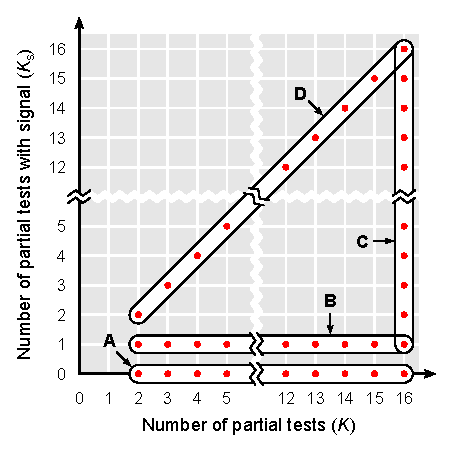
\includegraphics{images/simulations.eps}}
\end{center}
\vspace{-3mm}
\caption{The simulations \textsc{a}--\textsc{d}. Each was constructed with a set of $K$ partial tests, a number of which ($K_s$) had synthetic signal added.}
\label{fig:simulations}
\end{figure}

The response variables $\mathbf{Y}$ had size $N \times K$, $N=20$, that is, simulating measurements for 20 subjects, each with $K$ image modalities (partial tests). Each modality was simulated as having 500 points, these representing, for instance, voxels or vertices. The errors were simulated following either a Gaussian distribution with zero mean and unit variance, or a Weibull distribution, with scale parameter 1 and shape parameter $\sfrac{1}{3}$, shifted and scaled so as to have expected zero mean and unit variance. The response data were constructed by adding to the errors the simulated effects --- either no signal, or a signal with strength callibrated to yield an approximate power of 50\% with Gaussian errors, irrespective of the sample size, as described above for the simulations that tested the validity of the modified \textsc{npc}; for the Weibull errors, the signal was further decreased, in all these four simulations, by a factor $\sfrac{5}{8}$, thus minimising saturation at maximum power in simulation \textsc{d}. The actual effect was coded in the first regressor only, which was constructed as a set of random values following a Gaussian distribution with zero mean and unit variance; the second regressor was modelled as an intercept.

The simulated data was tested using 500 shufflings (permutations, sign-flippings, and permutations with sign-flippings). For all the simulations, the whole process was repeated 100 times, allowing histograms of p-values to be constructed, as well as to estimate the variability around the heights of the histogram bars. Confidence intervals (95\%) were computed for the empirical error rates and power using the Wilson method.

\subsection{Example: Pain study}

While the proposed correction for the \textsc{mtp-ii} has a predictable consequence, that is, controlling the familywise error rate at the nominal level, the combination of modalities, designs, and contrasts may not be quite as obvious. In this section we show a re-analysis of the data of the pain study by \citet{Brooks2005}. In brief, subjects received, in separate tests, painful, hot stimuli in the right side of the face (just below the lower lip), dorsum of the right hand, and dorsum of the right foot. The objective was to investigate somatotopic organisation of the pain response in the insular cortex using \textsc{fmri}, and the complete experimental details, stimulation and imaging acquisition protocols, analysis and conclusions can be found in the original publication. Here we sought to identify, at the group level, in standard space, areas within the insula that jointly respond to hot painful stimuli across the three topologically distinct body regions. We used the modified \textsc{npc}, comparing the combining functions of Tippett, Fisher, Stouffer and Mudholkar--George, as well as the Hotelling's $T^2$ statistic, and an \textsc{iut} (conjunction). At the group level, the design is a one-sample t-test, for which only sign flippings can be used to test the null hypothesis. We used twelve of the original subjects, and performed exhaustively all the 4096 sign flippings possible.

\section{Results}

A large number of plots and tables were produced and are shown in the Supplementary Material. The Figures below contain only the most representative results, that are sufficient to highlight the major points.

\subsection{Validity of the modified \textsc{npc}}

Both the original and the modified \textsc{npc} methods controlled the error rates at exactly the level of the test. Such validity was not limited to $\alpha=0.05$, and the histograms of uncorrected p-values under complete absence of signal were flat throughout the whole $[0, 1]$ interval for both the original and modified \textsc{npc} methods, using either the Tippett or the Fisher combining functions. A representative subset of the results, for the Fisher method only, and for sample sizes $N = \{$8, 12, 20, 40$\}$, is shown in Figure~\ref{fig:validity_hist}.

\begin{figure}[p]
\begin{center}
\centerline{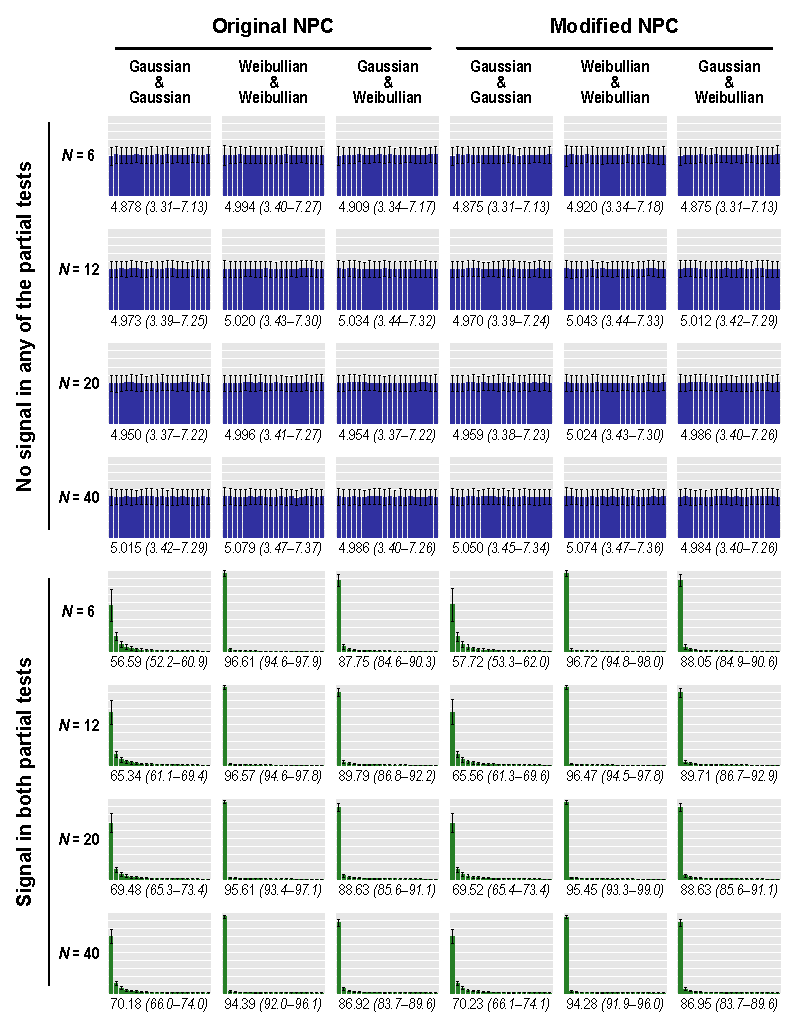
\includegraphics{images/validity_hist.eps}}
\end{center}
\vspace{-3mm}
\caption{Histograms of frequency of p-values for the simulation without signal in either of the two partial tests (upper panel, blue bars) or with signal in both (lower panel, green bars). The values below each plot indicate the height (in percentage) of the first bar, which corresponds to p-values smaller than or equal to 0.05, along with the confidence interval (95\%, italic). Both original and modified \textsc{npc} methods controlled the error rates at the nominal level, and produced flat histograms in the absence of signal. The histograms suggest similar power for both approaches. See also the Supplemental Material.}
\label{fig:validity_hist}
\end{figure}

When considering the uncorrected p-values, the modified \textsc{npc} yielded a mostly negligible increase in power when compared to the original \textsc{npc}, with the difference always within the 95\% confidence interval. Although this slight gain can be hardly observed in the histograms and Bland--Altman plots for the uncorrected p-values, they are clearly visible in the Bland--Altman plots for the p-values corrected across the 500 tests. In these plots, the predominance of smaller (towards more significant) p-values can be seen as a positive difference between the original and modified \textsc{npc} p-values. A representative subset of the results is shown in Figure~\ref{fig:validity_ba}.

\begin{figure}[p]
\begin{center}
\centerline{\includegraphics{images/validity_ba.eps}}
\end{center}
\vspace{-3mm}
\caption{Bland--Altman plots comparing the original and modified \textsc{npc}, for both uncorrected and corrected p-values, without signal in either of the two partial tests (upper panel, blue dots) or with signal in both (lower panel, green dots). The values below each plot indicate the percentage of points within the 95\% confidence interval ellipsoid. For smaller sample sizes and non-Gaussian error distributions, the methods differ, but the differences become negligible as the sample size increases. In the presence of signal, the modification caused increases in power, particularly for the corrected p-values.}
\label{fig:validity_ba}
\end{figure}

\subsection{Performance of combined tests}

Representative results demonstrating the performance of the methods of Tippett, Fisher, Stouffer, Mudholkar--George, as well as Hotelling's $T^2$, is shown in Figure~\ref{fig:performance}. The remaining results are browseable in the Supplementary Material. In the absence of signal (simulation \textsc{a}), all combining functions controlled the error rate at the level of the test or below it, never above, thus confirming their validity. With normally distributed (Gaussian) errors, most functions yielded uniformly distributed p-values, although some functions seemed to converge towards uniformity only as the number of partial tests is increased; this was the case for the methods of Wilkinson, Zaykin, Dudbridge--Koeleman (\textsc{dtp}) and Jiang. With skewed (Weibullian) errors, the error rate was controlled at the test level with the use of permutations; with sign-flippings or permutations with sign-flippings, the combined results tended to be conservative, and more so for the Hotelling's $T^2$ statistics (and likewise the Wilks' $\lambda$).

\begin{figure}[p]
\begin{center}
\centerline{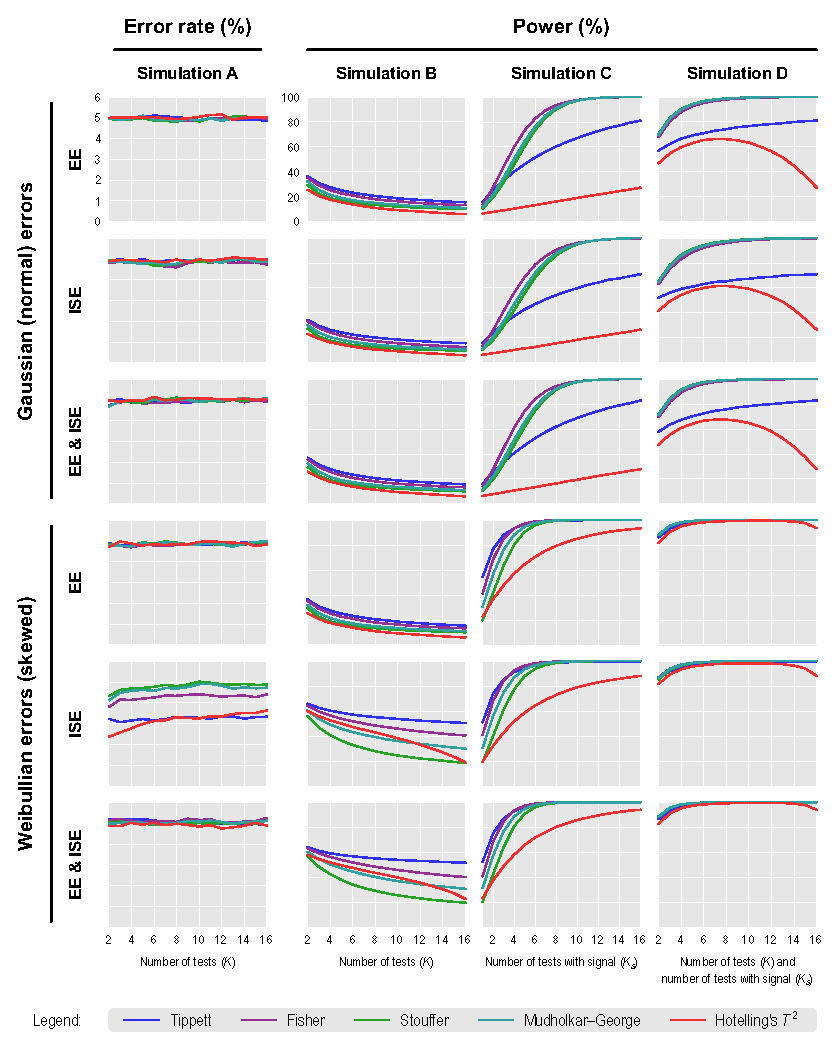
\includegraphics{images/performance.eps}}
\end{center}
\vspace{-3mm}
\caption{Performance of the modified \textsc{npc} with four representative combining functions (Tippett, Fisher, Stouffer, and Mudholkar--George) and of one \textsc{cmv} (Hotelling's $T^2$), using normal or skewed errors, and using permutations (\textsc{ee}), sign flippings (\textsc{ise}), or both. All resulted in error rates controlled at or below the level of the test. The Tippett and Fisher were generally the most powerful, with Tippett outperforming others with signal present in a small fraction of the tests, and with Fisher having the best power in the other settings.}
\label{fig:performance}
\end{figure}

With signal added to just one of the partial tests (simulation \textsc{b}), the method of Tippett was generally the most powerful, followed by the methods of Fisher and Dudbridge--Koeleman (both \textsc{rtp} and \textsc{dtp} variants). As the number of tests was increased, predictably, the power was reduced for all tests. The method of Stouffer did not in general have good performance with skewed errors, presumably because the dependence on $z$-statistics strengthens the dependence on the assumption of normality of the statistics for the partial tests in the modified \textsc{npc}. The \textsc{cmv} did not deliver a good performance either, being generally among the least powerful.

With the number of partial tests held fixed, as the number of tests with signal was increased (simulation \textsc{c}), the power of the method of Fisher increased more quickly than of the other methods, although when most of the partial tests had signal, most of the combining functions reached similar power, all close to 100\% for both normal or skewed errors. Hotelling's $T^2$ test was the considerably less powerful than any of the combining functions used with the modified \textsc{npc}.

As the total number of partial tests and the number of partial tests with signal were both increased (simulation \textsc{d}), almost all combined tests had similar power, and reached saturation (100\% power) quickly, particularly for the Weibullian errors, in which the calibration, even after reduction with the $\sfrac{5}{8}$ factor, yielded power above 50\% for each partial test. With Gaussian errors, in which calibration ensured average 50\% power, two tests had considerably lower sensitivity: Tippett's and Hotelling's $T^2$, the last with the remarkable result that power reached a peak, then began to fall as the number of tests kept increasing.

\subsection{Example: Pain study}

Using a conventional, mass univariate voxelwise tests, assessed through sign flippings, and after correction for multiple testing (\textsc{mtp-i}), only a few, sparse voxels could be identified at the group level for face, hand, and foot stimulation separately, in all cases with multiple distinct foci of activity observed bilaterally in the anterior and posterior insula. However, the joint analysis using the modified \textsc{npc} with Fisher, Stouffer and Mudholkar--George evidenced robust activity in the anterior insula bilaterally, posterior insula, secondary somatosensory cortex (\textsc{sii}), and a small focus of activity in the midbrain, in the periaqueductal gray area. The combining function of Tippett, however, did not identify these regions, presumably because this method is less sensitive than the others when signal is present in more than a single partial test, as suggested by the findings in the previous section.

\begin{figure}[p]
\begin{center}
\centerline{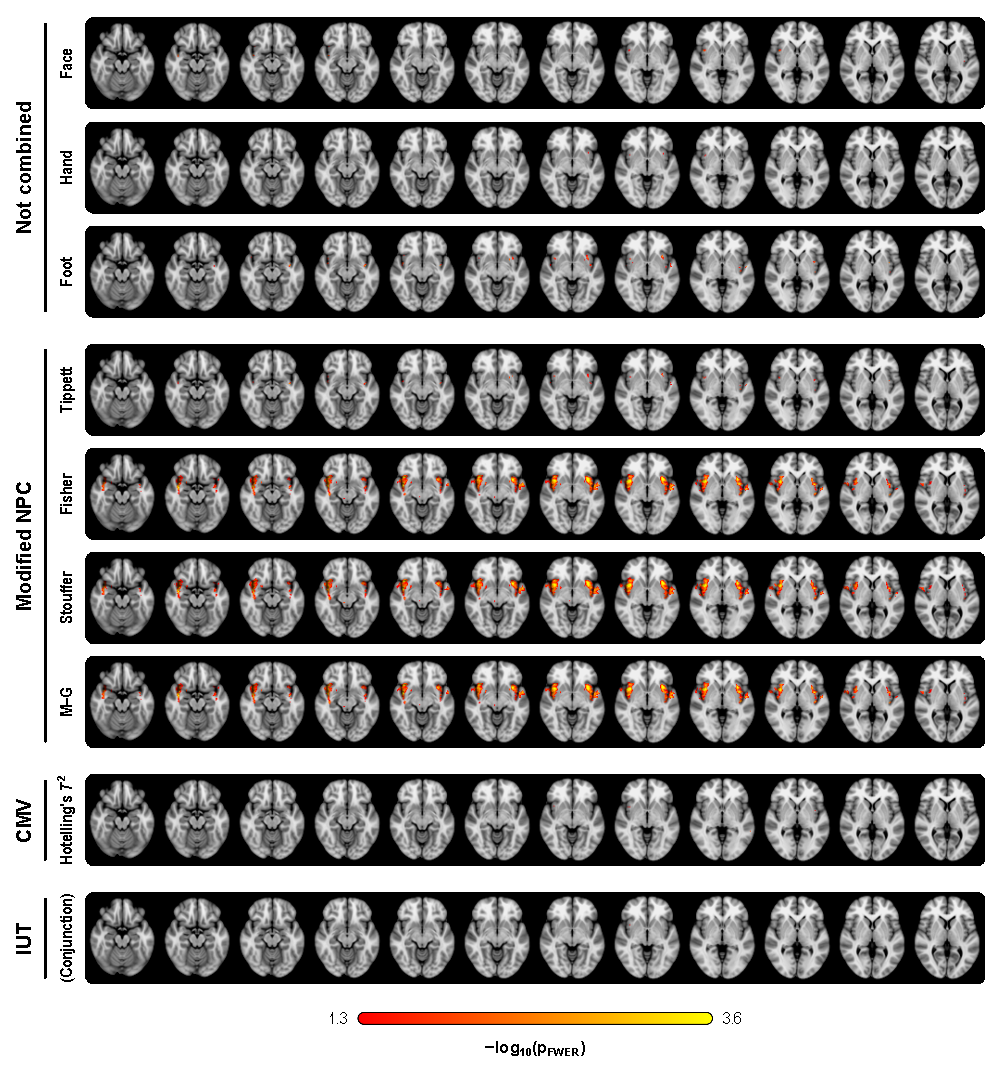
\includegraphics{images/pain.eps}}
\end{center}
\vspace{-9mm}
\caption{Without combination, and with correction across voxels (\textsc{mtp-i}), no significant results were observed at the group level for any of the three tests. Combination using the methods of Fisher, Stouffer and Mudholkar--George (M--G), however, evidenced bilateral activity in the insula in response to hot, painful stimulation. A classical multivariate test, Hotelling's $T^2$, as well as the Tippett method, failed to identify these areas. An intersection-union test (conjunction) could not locate significant results; such a test has a different null hypothesis that distinguishes it from the others. Images are in radiological orientation. For cluster-level results, comparable to \citet{Brooks2005}, see the Supplementary Material.}
\label{fig:pain}
\end{figure}

The Hotelling's $T^2$ was not able to identify these regions, with almost negligible, sparse, single-voxel findings in the anterior insula, bilaterally. The conjunction test, that has a different \textsc{jnh}, and searches for areas where all partial tests are significant, identified a single, barely visible, isolated voxel in the right anterior insula.

The above results are shown in Figure~\ref{fig:pain}. Cluster-level maps that can directly be compared to the original findings of \citet{Brooks2005} are shown in the Supplementary Material.

\section{Discussion}

\subsection{Validity of the modified \textsc{npc}}

The modified \textsc{npc} combines u-values, which are simply parametric p-values here renamed to avoid confusion. The renaming, however, emphasises the fact that the conversion to u-values via a parametric approximation should only be seen as a data transformation, in which the interpretation as a p-value is not preserved due to untenable assumptions. The combination method continues to be non-parametric as the combined statistic is assessed non-parametrically. More importantly, irrespective of the validity of parametric assumptions, any dependence between the tests is accounted for, implicitly, by the combination procedure, without the need of any modelling that could, at best, introduce complex and perhaps untenable assumptions, and at worst, be completely intractable.

The results suggest that, even in the cases in which the modified \textsc{npc} could have failed, i.e., with small sample sizes and different distributions, the combined statistic controlled the error rate at the level of the test. This control, maintained even in such difficult scenarios, suggests that the modified \textsc{npc} controls the error rates in general. The results also suggest that the modification increases power, even if such increase is minute in some scenarios. The Bland--Altman plots indicate that gains in sensitivity are more pronounced in the results corrected for the \textsc{mtp-i}, suggesting that the modified method is appropriate not merely due to its expediency for imaging applications, but also for having increased sensitivity compared to the original \textsc{npc}.

\subsection{Performance of combined tests}

The results also demonstrate that the \textsc{npc} method is more powerful than the Hotelling's $T^2$. The superiority of combined permutation tests when compared to classical multivariate tests has been observed in the literature \citep{Blair1994}, and the fact that power increases as the number of partial tests with signal increases is one of its most remarkable features. While \textsc{cmv} depends on the positive-definiteness of the covariance matrix of the vectors of residuals, such limitation does not apply to \textsc{npc} \citep{Pesarin2010_finite}. As a consequence, although in the comparisons only the Hotelling's $T^2$ and the Wilks' $\lambda$ statistics were used (in the simulations, $\mathsf{rank}\left(\mathbf{C}\right) = 1$), and had their p-values assessed through permutations, similar behaviour can be expected when using other \textsc{cmv}s, such as Pillai's trace (and with $\mathsf{rank}\left(\mathbf{C}\right) > 1$). With effect, \textsc{npc} can be used even when the number of variables equals or even greatly exceeds the number of observations, that is, when $K \geqslant N$. In the results shown in Figure~\ref{fig:performance}, this can be noted as a reduction in power that can be seen with the Hotelling's $T^2$, particularly for simulation \textsc{d}, and this is the case even considering that the test is assessed through permutations.

Regarding the different combining functions, the simulations show that the method of Tippett is the most powerful when signal is present in only a small fraction of the partial tests. For other cases, other combining functions, particularly that of Fisher, tend to be considerably more powerful.

The results also indicate that the use of sign flipping when the errors are not symmetric (a violation of assumptions) tends to produce a conservative test, with error rates below the nominal level, even if the power eventually remained unaltered when compared with permutations. While permutations together with sign flippings did alleviate conservativeness, at least for the Tippett method, the error rate remained below the nominal level. In general, if the errors are known to be skewed, only permutations should be used; if sign flippings are used, the error rate can be expected to be below the nominal level.

\subsection{Interpretation of combined tests}

The key aspect of the \textsc{npc} is that these tests seek to identify, \emph{on the aggregate} of the partial tests, a measure of evidence against the \textsc{jnh}, even if only some or none of them can be considered significant when seen in isolation, just as originally pointed out by \citet{Fisher1932}:

\begin{quote}
\emph{When a number of quite independent tests of significance have been made, it sometimes happens that although few or none can be claimed individually as significant, yet the aggregate gives an impression that the probabilities are on the whole lower than would often have been obtained by chance. It is sometimes desired (\ldots) to obtain a single test of the significance of the aggregate.}
\end{quote}

\noindent
This is the logic and interpretation of all of these combining statistics, with the exception of the conjunction inference. Combination is known to be able to answer questions that could otherwise not be answered be at all, or be answered less accurately if each information source were considered separately \citep{Draper1992}. Here the simulations and the pain study exemplify these aspects, and the improved sensitivity compared to each partial test when seen in separate.

As they depend on fewer assumptions than classical multivariate tests, \textsc{npc} can be considered whenever the validity of the former cannot be guaranteed. Even when parametric \textsc{cmv} assumptions hold, note that the \textsc{npc} can have superior power when sample size is small and prevents precise estimation of a covariance.

It should be noted that the aggregation of information follows a different principle than using different measurements separately to interrogate particular aspects of the brain (or of any other experiment or physiological phenomenon). Used judiciously, \textsc{npc} provides a complete framework that can be used for both the aggregate and for the correction of tests separately, with the valuable feature of being based on minimal assumptions.

\subsection{Correction over contrasts and over modalities}

Correction over contrasts using synchronised permutations provides a novel solution to the multiple comparisons problem for certain common experimental designs, in particular, for the popular one-way \textsc{anova} layout, that is, when the means of multiple groups are compared. The classical Fisher's protected least significant difference (\textsc{lsd}), that consists of performing an omnibus $F$-test and only proceeding to the group-wise post hoc tests if this initial test is significant, is known to fail to control the error rate if there are more than just three groups \citep{Hayter1986, Hsu1996, Meier2006}, and the failure can be by a wide margin, that grows as the number of groups being compared increases. Even though the same may not happen with other correction methods \citep[e.g., Tukey's range test,][]{Tukey1949}, the correction done non-parametrically also renders these older, parametric methods, redundant.

The correction over contrasts further obviates methods that are based on what has been termed ``logical constraints'' among hypotheses \citep{Shaffer1986, Hochberg1987}, as the dependencies among the tests are implicitly taken into account by the correction using the distribution of the extremum across contrasts, with or without concomitant combination or correction across multiple $K$ variables. In fact, the use of an omnibus $F$-test as a way to guard against multiple testing becomes quite unnecessary.

In the same manner, while combination across multiple modalities is a powerful substitute for classical multivariate tests as shown earlier, the correction across such modalities can replace the post hoc tests that are usually performed after significant results are found with \textsc{cmv}s.

\subsection{Pain study}

Joint significance is an important consideration when trying to interpret data such as these, that are distinct in some aspects (here, the topography of the stimulation), but similar in others (here, the type of stimulation, hot and painful), strengthening the case for distinct representations in some brain regions, but not in others. In terms of identifying areas with significant joint activity, the results suggest involvement of large portions of the anterior insula and secondary somatosensory cortex. The Fisher, Stouffer and Mudholkar--George combining functions were particularly successful in recovering a small area of activity in the midbrain and periaqueductal gray area that would be expected from previous studies on pain \citep{Reynolds1969, Petrovic2002, Tracey2002, Roy2014}, but that could not be located from the original, non-combined data.

\subsection{Relationship with meta-analysis}

Most of the combining functions shown in Table~\ref{tab:comparison} were originally defined based on p-values, and some of them are popular in meta-analyses, such as those of Fisher and Stouffer \citep{Borenstein2009}. Although there are commonalities between these meta-analytical methods and \textsc{npc}, it is worth emphasising that the two constitute distinct approaches to entirely different problems. In the \textsc{npc}, the objective is to interrogate joint significance across the multiple observed variables (or multiple designs and contrasts if these are instead combined) when the data for each individual observation is readily available to the researcher. Meta-analyses methods based on p-values, while sometimes using the same combining functions, attempt to identify a joint effect across multiple studies that not have necessarily been performed on the same experimental units, and when the data for the individual observations are not available. Moreover, the p-value of the combined statistic in the \textsc{npc} is produced through permutations, a procedure that is not available for ordinary meta-analytical methods. 

The fact that \textsc{npc} and meta-analysis form different approaches to separate problems also imply that certain criticisms levelled at the use of certain combined functions in the context of meta-analysis do not extend trivially to \textsc{npc}. As the simulations show, various of the combining functions more recently developed did not in general outperform older combining methods, such as Fisher and Stouffer, even though these were developed precisely for that purpose, in the context of meta-analyses, or for problems framed as such.

\section{Conclusion}

We proposed and evaluated a modified version of Non-Parametric Combination that is feasible and useful for imaging applications, and serves as a more powerful alternative to classical multivariate tests. We presented and discussed aspects related multiple testing problems in brain imaging, and proposed a single framework that addresses all these concerns at once. We showed that combination and correction of multiple imaging modalities, designs, and contrasts, are related to each other in the logic of their implementation, and also through the use of the simplest and the oldest of the combining functions, attributed to Tippett.
